\documentclass[12pt]{extarticle} 
%\usepackage{unicode-math}
\usepackage{amsmath,amsfonts,amssymb,amsthm,graphicx,xcolor,natbib,booktabs,tabularx}
%\usepackage[paperwidth=126mm, paperheight=96mm, top=5mm, bottom=5mm, right=5mm, left=5mm]{geometry}
\usepackage[margin=1cm,footskip=5mm]{geometry}
\pagenumbering{gobble}

\usepackage[inline]{enumitem}
\usepackage[BoldFont,SlantFont]{xeCJK}  
\xeCJKsetemboldenfactor{2}
\setCJKmainfont{cwTeX Q Yuan Medium}
\newcommand{\ds}{\displaystyle}
\newcommand{\ie}{\;\Longrightarrow\;}
\newcommand{\ifff}{\;\Longleftrightarrow\;}
\newcommand{\orr}{\;\vee\;}
\newcommand{\andd}{\;\wedge\;}
\newcommand{\mi}{\mathrm{i}}
\newcommand{\llt}{\left\langle}
\newcommand{\rgt}{\right\rangle}
\DeclareMathOperator*{\dom}{dom}
\DeclareMathOperator*{\codom}{codom}
\DeclareMathOperator*{\ran}{ran}
\DeclareMathOperator*{\sgn}{sgn}
\DeclareMathOperator*{\degr}{deg}
\newcommand{\floor}[1]{\lfloor #1 \rfloor}
\newcommand{\ceil}[1]{\lceil #1 \rceil}
\newcommand{\proj}[2]{\mathrm{proj}_{\,#2}\,#1}

% figure --> 圖
\renewcommand{\appendixname}{附錄}
\renewcommand{\figurename}{圖}
\renewcommand{\tablename}{表}
\renewcommand{\refname}{參考文獻}

\usepackage{hyperref}
\hypersetup{
    colorlinks,
    linkcolor={red!50!black},
    citecolor={blue!60!black},
    urlcolor={blue!60!black}
    %urlcolor={blue!80!black}
}

\theoremstyle{definition}
\newtheorem*{dfn}{定義}
\newtheorem*{prp}{性質}
\newtheorem*{fact}{結論}
\newtheorem*{thm}{定理}
\newtheorem*{ex}{例}
\newtheorem*{sol}{解}
\newtheorem*{prf}{證}
\newtheorem*{rmk}{註}
\newtheorem*{exe}{習題}

%\setenumerate{label=(\roman*),itemsep=1pt,topsep=3pt}
\newcommand{\myline}{\noindent\makebox[\linewidth]{\rule{\paperwidth}{0.4pt}}}
%\newcommand{\myline}{\textcolor[RGB]{220,220,220}{\rule{\linewidth}{1pt}}}

\usepackage{pgfplots}
\usetikzlibrary{arrows.meta,angles,quotes,patterns}
% axis style, ticks, etc
\pgfplotsset{every axis/.append style={
                   label style={font=\fontsize{4}{4}\selectfont},
                   tick label style={font=\fontsize{4}{4}\selectfont}  
               },
            }
\renewcommand\tabularxcolumn[1]{m{#1}}

%%%%%%%%%%%%%%%%%%%%%%%%%%%%%%%%%%%%%%%%%%%%%%%%%%%%%%%%%%%%%%%%%%%%%

\usepackage{multicol}
\usepackage{ifthen}
\tikzstyle{vertex}=[shape=circle, minimum size=2mm, inner sep=0, fill]
\tikzstyle{opendot}=[shape=circle, minimum size=2mm, inner sep=0, fill=white, draw]
\newcommand{\myaxis}[7][help lines]{%[formatting of lines]{xlabel}{xleft}{xright}{ylabel}{yleft}{yright}
	\ifthenelse{\lengthtest{#3 pt=0 pt}}{}{
		\draw[ <-,#1] (-#3,0)--(0,0);
		}
	\ifthenelse{\lengthtest{#4 pt=0 pt}}{
		\draw[#1] (0,0)node[right]{$#2$};}{
		\draw[ ->,#1] (0,0)--(#4,0)node[right]{$#2$};
		}
	\ifthenelse{\lengthtest{#6 pt= 0 pt}}{
		}{
		\draw[ <-,#1] (0,-#6)--(0,0);}
	\ifthenelse{\lengthtest{#7 pt= 0 pt}}{
		\draw[#1] (0,0)node[above]{$#5$};
		}{
		\draw[ ->,#1] (0,0)--(0,#7)node[above]{$#5$};}
}

% colorblind-friendly palette
% mixed colours: CB sees contrasting grays
\definecolor{M1}{RGB}{0,0,0}
\definecolor{M2}{RGB}{0,73,73}
\definecolor{M3}{RGB}{0,146,146}
\definecolor{M4}{RGB}{255,109,182}
\definecolor{M5}{RGB}{255,182,119}
% cool colours: CB sees contrasting blues
\definecolor{C1}{RGB}{73,0,146}
\definecolor{C2}{RGB}{0,109,219}
\definecolor{C3}{RGB}{182,109,255}
\definecolor{C4}{RGB}{109,182,255}
\definecolor{C5}{RGB}{182,219,255}
% warm colours: CB sees contrasting yellow
\definecolor{W1}{RGB}{146,0,0}
\definecolor{W2}{RGB}{146,73,0}
\definecolor{W3}{RGB}{219,209,0}
\definecolor{W4}{RGB}{36,255,36}
\definecolor{W5}{RGB}{255,255,109}

%%%%%%%%%%%%%%%%%%%%%%%%%%%%%%%%%%%%%%%%%%%%%%%%%%%%%%%%%%%%%
% from clp3

\newcommand{\vr}{\mathbf{r}}
\newcommand{\vR}{\mathbf{R}}
\newcommand{\vv}{\mathbf{v}}
\newcommand{\va}{\mathbf{a}}
\newcommand{\vb}{\mathbf{b}}
\newcommand{\vc}{\mathbf{c}}
\newcommand{\vd}{\mathbf{d}}
\newcommand{\ve}{\mathbf{e}}
\newcommand{\vC}{\mathbf{C}}
\newcommand{\vp}{\mathbf{p}}
\newcommand{\vn}{\mathbf{n}}
\newcommand{\vu}{\mathbf{u}}
%\newcommand{\vv}{\mathbf{v}}
\newcommand{\vV}{\mathbf{V}}
\newcommand{\vx}{\mathbf{x}}
\newcommand{\vX}{\mathbf{X}}
\newcommand{\vy}{\mathbf{y}}
\newcommand{\vz}{\mathbf{z}}
\newcommand{\vF}{\mathbf{F}}
\newcommand{\vG}{\mathbf{G}}
\newcommand{\vH}{\mathbf{H}}
\newcommand{\vM}{\mathbf{M}}
\newcommand{\vT}{\mathbf{T}}
\newcommand{\vN}{\mathbf{N}}
\newcommand{\vL}{\mathbf{L}}
\newcommand{\vA}{\mathbf{A}}
\newcommand{\vB}{\mathbf{B}}
\newcommand{\vD}{\mathbf{D}}
\newcommand{\vE}{\mathbf{E}}
\newcommand{\vJ}{\mathbf{J}}
\newcommand{\vZero}{\mathbf{0}}
\newcommand{\vPhi}{\mathbf{\Phi}}
\newcommand{\vOmega}{\mathbf{\Omega}}
\newcommand{\vTheta}{\mathbf{\Theta}}
\newcommand{\cA}{\mathcal{A}}
\newcommand{\cB}{\mathcal{B}}
\newcommand{\cM}{\mathcal{M}}
\newcommand{\cO}{\mathcal{O}}
\newcommand{\cR}{\mathcal{R}}
\newcommand{\cS}{\mathcal{S}}
\newcommand{\cT}{\mathcal{T}}
\newcommand{\cU}{\mathcal{U}}
\newcommand{\cV}{\mathcal{V}}
\newcommand{\cW}{\mathcal{W}}
\newcommand{\cX}{\mathcal{X}}

%\newcommand{\hi}{\hat{\mathbf{i}}}
%\newcommand{\hj}{\hat{\mathbf{j}}}
\newcommand{\hi}{\widehat{\pmb{\imath}}}
\newcommand{\hj}{\widehat{\pmb{\jmath}}}
\newcommand{\hk}{\widehat{\mathbf{k}}}
\newcommand{\hn}{\widehat{\mathbf{n}}}
\newcommand{\hr}{\widehat{\mathbf{r}}}
\newcommand{\hvt}{\widehat{\mathbf{t}}}
\newcommand{\hN}{\widehat{\mathbf{N}}}
\newcommand{\vth}{{\pmb{\theta}}}
\newcommand{\vTh}{{\pmb{\Theta}}}
%\newcommand{\vnabla}{\pmb{\nabla}}
\newcommand{\vnabla}{   { \mathchoice{\pmb{\nabla}}
                            {\pmb{\nabla}}
                            {\pmb{\scriptstyle\nabla}}
                            {\pmb{\scriptscriptstyle\nabla}} }   }
\newcommand{\ha}[1]{\mathbf{\hat e}^{(#1)}}

\newcommand{\bbbc}{\mathbb{C}}

\newcommand{\Om}{\Omega}
\newcommand{\om}{\omega}
\newcommand{\vOm}{\pmb{\Omega}}
\newcommand{\svOm}{\pmb{\scriptsize\Omega}}
\newcommand{\al}{\alpha}
\newcommand{\be}{\beta}
\newcommand{\de}{\delta}
\newcommand{\ga}{\gamma}
\newcommand{\ka}{\kappa}
\newcommand{\la}{\lambda}

\newcommand{\cC}{\mathcal{C}}
\newcommand{\bbbone}{\mathbb{1}}

\def\tr{\mathop{\rm tr}}
\newcommand{\Atop}[2]{\genfrac{}{}{0pt}{}{#1}{#2}}

%\newcommand{\pdiff}[2]{ \frac{\partial\hfil#1\hfil}{\partial #2}}
\newcommand{\pdiff}[2]{\frac{\partial #1}{\partial #2}}
\newcommand{\pdifft}[2]{\frac{\partial^2 #1}{\partial #2^2}}
\newcommand{\dblInt}{\iint}
\newcommand{\tripInt}{\iiint}
%\newcommand{\dblInt}{\int\!\!\int}
%\newcommand{\tripInt}{\int\!\!\!\int\!\!\!\int}
%\newcommand{\dblInt}{\mathop{\int\!\!\!\int}}
%\newcommand{\tripInt}{\mathop{\int\!\!\!\int\!\!\!\int}}

\newcommand{\Set}[2]{\big\{ \ #1\ \big|\ #2\ \big\}}
\newcommand{\rhof}{{\rho_{\!{\scriptscriptstyle f}}}}
\newcommand{\rhob}{{\rho_{{\scriptscriptstyle b}}}}

\renewcommand{\neg}{ {\sim} }
\newcommand{\limp}{ {\;\Rightarrow\;} }
\newcommand{\nimp}{ {\;\not\Rightarrow\;} }
\newcommand{\liff}{ {\;\Leftrightarrow\;} }
\newcommand{\niff}{ {\;\not\Leftrightarrow\;} }

\newcommand{\st}{ {\mbox{ s.t. }} }
\newcommand{\es}{ {\varnothing}}
\newcommand{\pow}[1]{ \mathcal{P}\left(#1\right) }
\newcommand{\set}[1]{ \left\{#1\right\} }

\newcommand{\bbbn}{\mathbb{N}}
\newcommand{\bbbr}{\mathbb{R}}
\newcommand{\bbbp}{\mathbb{P}}
\newcommand{\De}{\Delta}
\newcommand{\cD}{\mathcal{D}}
\newcommand{\cP}{\mathcal{P}}
\newcommand{\cI}{\mathcal{I}}
\newcommand{\veps}{\varepsilon}
\newcommand{\dee}[1]{\mathrm{d}#1}

\newcommand{\bdiff}[2]{ \frac{\mathrm{d}}{\mathrm{d}#2} \left( #1 \right)}
\newcommand{\ddiff}[3]{ \frac{\mathrm{d}^#1#2}{\mathrm{d}{#3}^#1}}
\newcommand{\half}{\tfrac{1}{2}}
\newcommand{\diff}[2]{\frac{\mathrm{d} #1}{\mathrm{d} #2}}
\newcommand{\difftwo}[2]{\frac{\mathrm{d^2} #1}{\mathrm{d}{#2}^2}}

%%%%%%%%%%%%%%%%%%%%%%%%%%%%%%%%%%%%%%%%%%%%%%%%%%%%%%%%%%%%%%%%%%%%%

\usepackage{fancyhdr}
\fancypagestyle{firststyle} {
   \fancyhf{}
   \fancyfoot[R]{\footnotesize \DTMnow}
   \renewcommand{\headrulewidth}{0pt} 
}
\usepackage{datetime2}

\usepackage{nicefrac}
\newcommand{\eqover}[1]{}

\begin{document}
\title{\texorpdfstring{\vspace{-16mm} 第五章\ \ 偏微分}{第五章\ \ 偏微分}} 
\author{\vspace{-5em}}
\date{\vspace{-5em}}
\maketitle
\thispagestyle{firststyle}

\section*{5.0 微積分函數分類}
\setlength{\columnsep}{-20mm}
\begin{multicols}{2}
  \begin{enumerate}\setlength{\itemsep}{0pt}
    \item 單變數函數: $\mathbb{R}\to\mathbb{R}$
    \item 向量值函數: $\mathbb{R}\to\mathbb{R}^n$, $n > 1$ (5.2)
    \item 多變數函數: $\mathbb{R}^n\to\mathbb{R}$, $n > 1$ (5.3)
    \item 多變數向量值函數: $\mathbb{R}^n\to\mathbb{R}^m$, $m$, $n > 1$
  \end{enumerate}
\end{multicols}

\section*{5.1 空間向量}

\begin{dfn}[符號]
  \setlength{\columnsep}{10mm}
  \begin{multicols}{2}
    \begin{itemize}\setlength{\itemsep}{0pt}
      \item 向量: $\va$, $\vx$
      \item 分量形: $\va = \llt a_1,\,a_2,\,a_3\rgt$, $a_1$, $a_2$, $a_3\in\mathbb{R}$; $\va\in\mathbb{R}^3$. 
      \item 長度: $|\va| = |\llt a_1,\,a_2,\,a_3 \rgt| = \sqrt{a_1^2 + a_2^2 + a_3^2}$. 
      \item 三維直角座標系單位向量: $\hi = \llt 1,\,0,\,0\rgt$, $\hj = \llt 0,\,1,\,0\rgt$, $\hk = \llt 0,\,0,\,1\rgt$
      \item $\va = \llt a_1,\,a_2,\,a_3\rgt \equiv a_1\,\hi + a_2\,\hj + a_3\,\hk$
      \item $\vZero = \llt 0,\,0,\ldots,0\rgt$
    \end{itemize}
  \end{multicols}
\end{dfn}

\begin{dfn}[內積 / 點積]
  給定 $n$ ($n\geqslant 2$) 維向量 $\va = \llt a_1,\,a_2,\,\ldots,\,a_n\rgt$, $\vb = \llt b_1,\,b_2,\,\ldots,\,b_n\rgt$, 則 $\va$ 與 $\vb$ 的內積 / 點積 (inner product / dot product) 定義為 $\ds\va\cdot\vb = \sum_{i = 1}^n a_i\,b_i$. 
\end{dfn}

\begin{prp} 給定 $\va$, $\vb$, $\vc\in\mathbb{R}^n$, $n\geqslant 2$, $s\in\mathbb{R}$. 則
  \begin{itemize}\setlength{\itemsep}{0pt}
    \item $\va\cdot\vb = |\va|\,|\vb|\,\cos\theta$, $0\leqslant\theta\leqslant\pi$ 為 $\va$ 與 $\vb$ 的夾角. 
  \end{itemize}
  且
  \setlength{\columnsep}{-20mm}
  \begin{multicols}{2}
    \begin{enumerate}\setlength{\itemsep}{0pt}
      \item $\va\cdot\va = |\va|^2$
      \item $\va\cdot\vb = \vb\cdot\va$
      \item $(s\va)\cdot\vb = s(\va\cdot\vb)$
      \item $\vZero\cdot\va = 0$
      \item $\va\cdot\vb = 0\ifff\va=\vZero\;\vee\;\vb = \vZero\;\vee\;\va\,\bot\,\vb$
      \item $\va\cdot(\vb + \vc) = \va\cdot\vb + \va\cdot\vc$, $(\va + \vb)\cdot\vc = \va\cdot\vc + \vb\cdot\vc$
    \end{enumerate}
  \end{multicols}
\end{prp}

\begin{prf}
  \begin{figure}[!htbp]
    \centering
    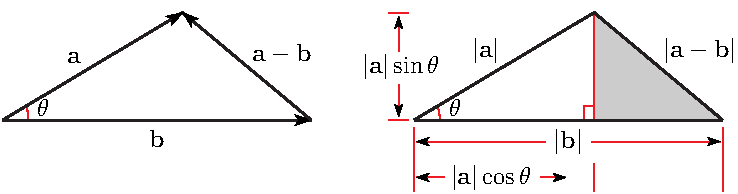
\includegraphics[scale=1,page=1]{fig/cosineB.pdf}
  \end{figure}
  由上圖, $\ds|\va-\vb|^2 = \big(|\vb|-|\va|\,\cos\theta\big)^2 + \big(|\va|\sin\theta\big)^2 = |\vb|^2 - 2\,|\va|\,|\vb|\,\cos\theta + |\va|^2\cos^2\theta + |\va|^2\sin^2\theta = |\vb|^2 - 2\,|\va|\,|\vb|\,\cos\theta + |\va|^2$, 又 $\ds|\va - \vb|^2 = (\va - \vb)\cdot(\va - \vb) = \va\cdot\va - \va\cdot\vb - \vb\cdot\va - \vb\cdot\vb = |\va|^2 + |\vb|^2 - 2\,\va\cdot\vb = |\vb|^2 - 2\,|\va|\,|\vb|\,\cos\theta + |\va|^2$, 故 $\va\cdot\vb = |\va|\,|\vb|\,\cos\theta$. 
\end{prf}

\begin{dfn}[投影] 
  給定向量 $\va$, $\vb$, 則 $\va$ 在 $\vb$ 方向上的投影 (projection) $\ds\proj{\va}{\vb}$ 定義為 $\ds\proj{\va}{\vb} = \frac{\va\cdot\vb}{|\vb|^2}\,\vb$. 
\end{dfn}

\begin{figure}[!htbp]
  \centering
  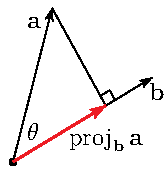
\includegraphics[scale=1,page=1]{fig/projA.pdf}
  \qquad\qquad
  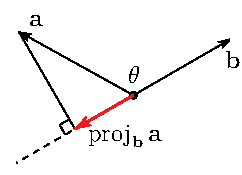
\includegraphics[scale=1,page=1]{fig/projB.pdf}
\end{figure}

\vspace{-5mm}
\begin{dfn}[外積 / 叉積] 
  給定三維向量 $\va = \llt a_1,\,a_2,\,a_3\rgt$, $\vb = \llt b_1,\,b_2,\,b_3\rgt$, 則 $\va$ 與 $\vb$ 的外積 / 叉積 (outer product / cross product) 定義為 $\ds\va\times\vb = \begin{vmatrix}\hi & \hj & \hk \\ a_1 & a_2 & a_3 \\ b_1 & b_2 & b_3\end{vmatrix} = \llt a_2b_3 - a_3b_2,\,a_3b_1 - a_1b_3,\,a_1b_2 - a_2b_1\rgt$. 
\end{dfn}

\begin{prp} 令 $\va$, $\vb$, $\vc\in\mathbb{R}^3$, $s\in\mathbb{R}$,
  \begin{itemize}\setlength{\itemsep}{0pt}
    \item $|\va\times\vb| = |\va|\,|\vb|\,\sin\theta$, $0\leqslant\theta\leqslant\pi$ 為 $\va$ 與 $\vb$ 的夾角; $|\va\times\vb|$ 為 $\va$ 與 $\vb$ 張成之平行四邊形面積. 
    \item $\va\times\vb = |\va|\,|\vb|\,\sin\theta\,\hn$, $0\leqslant\theta\leqslant\pi$ 為 $\va$ 與 $\vb$ 的夾角, $(\va,\,\vb,\,\hn)$ 滿足右手定則且 $|\hn| = 1$, $\hn\,\bot\,\va$, $\hn\,\bot\,\vb$.  
    \item $|\va\cdot(\vb\times\vc)|$ 為 $\va$, $\vb$, $\vc$ 張成之平行六面體體積. 
  \end{itemize}
  且
  \setlength{\columnsep}{-20mm}
  \begin{multicols}{2}
    \begin{enumerate}\setlength{\itemsep}{0pt}
      \item $\va\times\vb\;\bot\;\va$, $\va\times\vb\;\bot\;\vb$ 
      \item $\hi\times\hj = \hk$,\;$\hj\times\hk = \hi$,\;$\hk\times\hi = \hj$
      \item $\va\times\vb = \vZero\ifff \va=\vZero\;\vee\;\vb = \vZero\;\vee\;\va\,\parallel\,\vb$
      \item $\va\times\vb = -\vb\times\va$
      \item $(s\va)\times\vb = \va\times(s\vb) = s(\va\times\vb)$
      \item $\va\times(\vb + \vc) = \va\times\vb + \va\times\vc$
      \item $(\va + \vb)\times\vc = \va\times\vc + \vb\times\vc$
      \item $\va\cdot(\vb\times\vc) = \vb\cdot(\vc\times\va) = \vc\cdot(\va\times\vb)$
      \item $\va\times(\vb\times\vc) = \vb\,(\va\cdot\vc) - \vc\,(\va\cdot\vb)$ (baccab 規則)  
    \end{enumerate}
  \end{multicols}
\end{prp}
\vspace{-3mm}
\begin{figure}[!htbp]
  \centering
  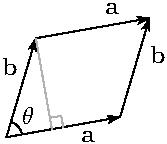
\includegraphics[scale=1,page=1]{fig/areaB.pdf}\qquad\qquad\qquad
  \raisebox{-0.05\height}{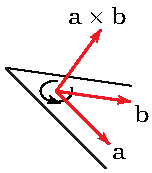
\includegraphics{fig/crossRR.pdf}}\qquad\qquad\qquad
  \raisebox{0.05\height}{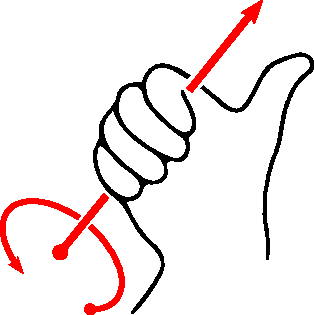
\includegraphics[scale=0.4]{fig/RHR.pdf}}
\end{figure}
\vspace{-5mm}
\begin{figure}[!htbp]
  \centering
  \raisebox{0.2\height}{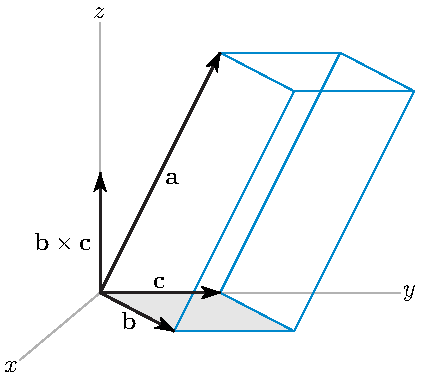
\includegraphics[scale=0.9]{fig/pipedVolumeEg.pdf}}\qquad\qquad
  \raisebox{0.4\height}{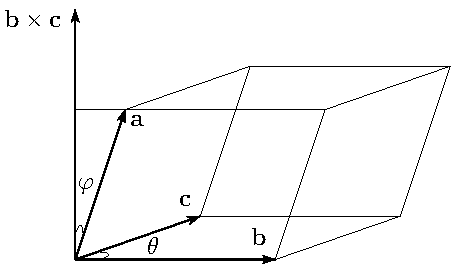
\includegraphics[scale=1.0]{fig/pipedVolume.pdf}}
\end{figure}
\vspace{-15mm}
\begin{prf}
  \begin{itemize}\setlength{\itemsep}{0pt}
    \item[]
    \item $\ds|\va\times\vb|^2 =\big(\va\times\vb\big)\cdot\big(\va\times\vb\big) = (a_2b_3-a_3b_2)^2 + (a_3b_1-a_1b_3)^2 + (a_1b_2-a_2b_1)^2 = a_2^2b_3^2-2a_2b_3a_3b_2+a_3^2b_2^2 +a_3^2b_1^2-2a_3b_1a_1b_3+a_1^2b_3^2 + a_1^2b_2^2-2a_1b_2a_2b_1+a_2^2b_1^2$, 而 $\ds|\va|^2\,|\vb|^2\sin^2\theta = |\va|^2\,|\vb|^2(1 - \cos^2\theta) = |\va|^2\,|\vb|^2 - (\va\cdot\vb)^2 = \big(a_1^2+a_2^2+a_3^2\big)\big(b_1^2+b_2^2+b_3^2\big)-\big(a_1b_1+a_2b_2+a_3b_3\big)^2 = a_1^2b_2^2+a_1^2b_3^2+a_2^2b_1^2+a_2^2b_3^2+a_3^2b_1^2+a_3^2b_2^2 - \big(2a_1b_1a_2b_2+2a_1b_1a_3b_3+2a_2b_2a_3b_3\big)$, 故 $|\va\times\vb|=|\va|\,|\vb|\sin\theta$ . 
    \item $\ds\va\cdot(\va\times\vb) = a_1(a_2 b_3 - a_3 b_2) + a_2(a_3 b_1 - a_1 b_3) + a_3(a_1 b_2 - a_2 b_1) = 0$, \\$\ds\vb\cdot(\va\times\vb) = b_1(a_2 b_3 - a_3 b_2) + b_2(a_3 b_1 - a_1 b_3) + b_3(a_1 b_2 - a_2 b_1) = 0$
    \item $\ds\va\cdot(\vb\times\vc) = \llt a_1,a_2,a_3\rgt\cdot\llt b_2c_3-b_3c_2\,,\, b_3c_1-b_1c_3\,,\, b_1c_2-b_2c_1\rgt = \textcolor{blue}{a_1b_2c_3}\textcolor{blue}{-a_1b_3c_2} + \textcolor{orange}{a_2b_3c_1}\textcolor{orange}{-a_2b_1c_3} + a_3b_1c_2 - a_3b_2c_1$, 又 $\ds(\va\times\vb)\cdot\vc =\llt a_2b_3-a_3b_2\,,\, a_3b_1-a_1b_3\,,\, a_1b_2-a_2b_1\rgt\cdot\llt c_1,c_2,c_3\rgt = \textcolor{orange}{a_2b_3c_1} - a_3b_2c_1 + a_3b_1c_2\textcolor{blue}{-a_1b_3c_2} + \textcolor{blue}{a_1b_2c_3}\textcolor{orange}{-a_2b_1c_3}$. \\另證: $\ds\va\cdot(\vb\times\vc) = \llt a_1,a_2,a_3\rgt\cdot\det\begin{vmatrix}\hi&\hj&\hk\\ b_1&b_2&b_3\\ c_1&c_2&c_3\end{vmatrix} = a_1\det\begin{vmatrix}b_2&b_3\\c_2&c_3\end{vmatrix} - a_2\det\begin{vmatrix}b_1&b_3\\c_1&c_3\end{vmatrix} + a_3\det\begin{vmatrix} b_1&b_2\\c_1&c_2\end{vmatrix} \\ = \det\begin{vmatrix}a_1&a_2&a_3\\b_1&b_2&b_3\\c_1&c_2&c_3\end{vmatrix}$, 而 $\ds(\va\times\vb)\cdot\vc = \det\begin{vmatrix}\hi&\hj&\hk\\a_1&a_2&a_3\\ b_1&b_2&b_3\end{vmatrix}\cdot\llt c_1,c_2,c_3\rgt = c_1\det\begin{vmatrix}a_2&a_3\\ b_2&b_3\end{vmatrix}-c_2\det\begin{vmatrix}a_1&a_3\\ b_1&b_3\end{vmatrix} + c_3\det\begin{vmatrix}a_1&a_2\\b_1&b_2\end{vmatrix} = \det\begin{vmatrix}c_1&c_2&c_3\\a_1&a_2&a_3\\b_1&b_2&b_3\end{vmatrix}$, 故 $\va\cdot(\vb\times\vc) = (\va\times\vb)\cdot\vc$. 
    \item $\ds\vb\times\vc = (b_2c_3-b_3c_2)\,\hi - (b_1c_3 - b_3c_1)\,\hj + (b_1c_2-b_2c_1)\,\hk$, 故 $\ds\va\times(\vb\times\vc) \\= \det\begin{vmatrix}\hi&\hj&\hk\\a_1&a_2&a_3\\b_2c_3 - b_3c_2&-b_1c_3 + b_3c_1&b_1c_2 - b_2c_1\end{vmatrix} = \hi\,\big(a_2(b_1c_2 - b_2c_1) - a_3(-b_1c_3 + b_3c_1)\big) - \hj\,\big(a_1(b_1c_2-b_2c_1)-a_3(b_2c_3-b_3c_2)\big) + \hk\,\big(a_1(-b_1c_3 + b_3c_1) - a_2(b_2c_3 - b_3c_2)\big)$. 而 $\ds\vb(\va\cdot\vc) - \vc(\va\cdot\vb) = (a_1c_1 + a_2c_2 + a_3c_3)(b_1\,\hi + b_2\,\hj + b_3\,\hk) - (a_1b_1 + a_2b_2 + a_3b_3)(c_1\,\hi + c_2\,\hj + c_3\,\hk) = \hi\,\big(\textcolor{blue}{a_1b_1c_1} + a_2b_1c_2 + a_3b_1c_3\textcolor{blue}{-a_1b_1c_1} - a_2b_2c_1 - a_3b_3c_1\big) +\hj\,\big(a_1b_2c_1 + \textcolor{blue}{a_2b_2c_2} + a_3b_2c_3 - a_1b_1c_2\textcolor{blue}{-a_2b_2c_2} - a_3b_3c_2\big) + \hk\,\big(a_1b_3c_1 + a_2b_3c_2 + \textcolor{blue}{a_3b_3c_3} - a_1b_1c_3 - a_2b_2c_3 \textcolor{blue}{-a_3b_3c_3}\big) = \hi\,(a_2b_1c_2+a_3b_1c_3-a_2b_2c_1-a_3b_3c_1) + \hj\,(a_1b_2c_1+a_3b_2c_3-a_1b_1c_2-a_3b_3c_2) + \hk\,(a_1b_3c_1+a_2b_3c_2-a_1b_1c_3-a_2b_2c_3)$, 故 $\va\times(\vb\times\vc) = \vb\,(\va\cdot\vc) - \vc\,(\va\cdot\vb)$. 
  \end{itemize}
\end{prf}

\begin{ex} 令 $\va$, $\vb$, $\vc$, $\vd\in\mathbb{R}^3$,
  \begin{multicols}{2}
    \begin{enumerate}\setlength{\itemsep}{0pt}
      \item $\va\times(\vb\times\vc) + \vb\times(\vc\times\va) + \vc\times(\va\times\vb) = 0$
      \item $(\va\times\vb)\cdot(\vc\times\vd) = (\va\cdot\vc)\,(\vb\cdot\vd) - (\va\cdot\vd)\,(\vb\cdot\vc)$
      \item $(\va\times\vb)\cdot\left((\vb\times\vc)\times(\vc\times\va) \right) = \left(\va\cdot(\vb\times\vc)\right)^2$
    \end{enumerate} 
  \end{multicols}
\end{ex}
\begin{sol}
  \begin{enumerate}\setlength{\itemsep}{0pt}
    \item[]
    \item $\va\times(\vb\times\vc) + \vb\times(\vc\times\va) + \vc\times(\va\times\vb) = \vb\,(\va\cdot\vc) - \vc\,(\va\cdot\vb) + \vc\,(\vb\cdot\va) - \va\,(\vb\cdot\vc) + \va\,(\vc\cdot\vb) - \vb\,(\vc\cdot\va) = 0$
    \item $(\va\times\vb)\cdot(\vc\times\vd) = \vc\cdot(\vd\times(\va\times\vb)) = \vc\cdot\left(\va\,(\vd\cdot\vb) - \vb\,(\vd\cdot\va)\right) = (\vc\cdot\va)\,(\vd\cdot\vb) - (\vc\cdot\vb)\,(\vd\cdot\va)  = (\va\cdot\vc)\,(\vb\cdot\vd) - (\va\cdot\vd)\,(\vb\cdot\vc)$
    \item $(\va\times\vb)\cdot\left((\vb\times\vc)\times(\vc\times\va)\right) = (\vb\times\vc)\cdot\left((\vc\times\va)\times(\va\times\vb)\right) = (\vb\times\vc)\cdot\left(\va\,\left((\vc\times\va)\cdot\vb\right) - \vb\,\left((\vc\times\va)\cdot\va\right)\right) = (\vb\times\vc)\cdot(\va\,\left((\vc\times\va)\cdot\vb\right)) = \left(\va\cdot(\vb\times\vc)\right)^2$
  \end{enumerate} 
\end{sol}

\begin{prp}[常用公式] 
  \begin{itemize}\setlength{\itemsep}{0pt}
    \item[]
    \item 點 $p = (p_1,\,p_2,\,p_3)$ 與平面 $ax + by + cz + d = 0$ 距離為 $\ds\frac{|a p_1 + b p_2 + c p_3 + d|}{\sqrt{a^2 + b^2 + c^2}}$. 
    \item 若 $\va = \llt a_1,\,a_2,\,a_3\rgt$, $\vb = \llt b_1,\,b_2,\,b_3\rgt$, $\vc = \llt c_1,\,c_2,\,c_3\rgt$, $\vd = \llt d_1,\,d_2,\,d_3\rgt$, 三維空間中兩直線 \\$\ds\llt a_1 + b_1\,s,\,a_2 + b_2\,s,\,a_3 + b_3\,s\rgt$, $\ds\llt c_1 + d_1\,t,\,c_2 + d_2\,t,\,c_3 + d_3\,t \rgt$, $s$, $t\in\mathbb{R}$ 之距離為 $\ds\frac{|(\va - \vc)\cdot(\vb\times\vd)|}{|\vb\times\vd|}$. 
  \end{itemize}
\end{prp}

\begin{sol}
  \begin{itemize}\setlength{\itemsep}{0pt}
    \item[]
    \item 平面 $S:\,ax + by + cz + d = 0$ 法向量為 $\vn = \llt a,\,b,\,c\rgt$; 點 $p = (p_1,\,p_2,\,p_3)$ 與投影至平面 $S$ 之點 $o = (x,\,y,\,z)$ 所形成之向量平行於 $\vn$, 故 $(x,\,y,\,z) = (p_1 + a\,t,\,p_2 + b\,t,\,p_3 + c\,t)$, $t\in\mathbb{R}$ 為待定常數. 又 $o$ 位於平面 $S$ 上, 故 $\ds a(p_1 + a\,t) + b(p_2 + b\,t) + c(p_3 + c\,t) + d = 0 \ie t = \frac{-(a p_1 + b p_2 + c p_3 + d)}{a^2 + b^2 + c^2}$, 所求距離 $\ds\overline{op} = |\llt a\,t,\,b\,t,\,c\,t\rgt| = \sqrt{a^2 + b^2 + c^2}\,|t| = \frac{|a p_1 + b p_2 + c p_3 + d|}{\sqrt{a^2 + b^2 + c^2}}$. 
    \item 兩直線點分別為 $\va$, $\vc$, 方向向量分別為 $\vb$, $\vd$; $\vb\times\vd$ 同時垂直於兩直線, 所求距離即為 $\ds|\proj{(\va - \vc)}{\vb\times\vd}| = \frac{|(\va - \vc)\cdot(\vb\times\vd)|}{|\vb\times\vd|}$. 
  \end{itemize}
\end{sol}

\section*{5.2 向量值函數}

\begin{dfn}
  向量值函數 $\vr(t):\mathbb{R}\to\mathbb{R}^n$, $n > 1$, 其微分為
  \begin{equation*}
    \vr'(t) =  \diff{\vr}{t}(t)=\lim_{h\to 0}\frac{\vr(t+h)-\vr(t)}{h}\qquad\qquad\qquad
    \raisebox{-25pt}[25pt][20pt]{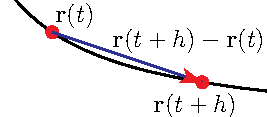
\includegraphics{fig/parCurveDerivA.pdf}}
  \end{equation*}
  若 $\ds\vr(t) = x(t)\,\hi + y(t)\,\hj + z(t)\,\hk$, 則 $\ds\vr'(t) = x'(t)\,\hi + y'(t)\,\hj + z'(t)\,\hk$. 
\end{dfn}

\begin{rmk}
  向量值函數多用在空間曲線表示式中: $\text{(曲線)}\,\equiv\,\text{(位置向量)}$. 
\end{rmk}

\begin{thm}[微分規則] 令 $\va(t)$, $\vb(t)$ 為 $t\in\bbbr$ 可微 $\bbbr^n$ 向量值函數, $\alpha$, $\beta\in\mathbb{R}$, $\ga(t)$, $s(t)$ 為 $t\in\bbbr$ 可微實函數, 則
  \begin{enumerate}\setlength{\itemsep}{0pt}
    \item (線性) $\ds\diff{}{t}\big(\alpha\,\va(t) + \beta\,\vb(t)\big) = \alpha\,\va'(t) + \beta\,\vb'(t)$
    \item (乘積) $\ds\diff{}{t}\big(\ga(t)\vb(t)\big) = \ga'(t)\vb(t)+\ga(t)\vb'(t)$
    \item (內積) $\ds\diff{}{t}\big(\va(t)\cdot\vb(t)\big) = \va'(t)\cdot\vb(t) + \va(t)\cdot\vb'(t)$
    \item (外積) $\ds\diff{}{t}\big(\va(t)\times\vb(t)\big) = \va'(t)\times\vb(t) + \va(t)\times\vb'(t)$
    \item (合成) $\ds\diff{}{t}\big(\va\big(s(t)\big)\big) = \va'\big(s(t)\big)\,s'(t)$
  \end{enumerate}
\end{thm}

\begin{ex}
  若 $\ds\vv(t) = \vr(t)\cdot(\vr'(t)\times\vr''(t))$, 證明 $\ds\vv'(t) = \vr(t)\cdot(\vr'(t)\times\vr'''(t))$.
\end{ex}

\begin{sol}
  $\ds\vv'(t) = \big(\vr(t)\cdot(\vr'(t)\times\vr''(t))\big)' = \vr'(t)\cdot(\vr'(t)\times\vr''(t)) + \vr(t)\cdot(\vr'(t)\times\vr''(t))' = \vr(t)\cdot(\vr'(t)\times\vr''(t))' = \vr(t)\cdot(\vr''(t)\times\vr''(t) + \vr'(t)\times\vr'''(t)) = \vr(t)\cdot(\vr'(t)\times\vr'''(t))$.
\end{sol}

\begin{prp} 給定曲線 $\vr(t)$.  
  \begin{enumerate}\setlength{\itemsep}{0pt}
    \item 令 $\widehat\vT(t)$ 為曲線在點 $\vr(t)$ 並指向 $t$ 遞增方向之單位切線向量, 則 $\ds\widehat\vT(t) = \frac{\vr'(t)}{|\vr'(t)|}$, $\vr'(t)\ne\vZero$. 
    \item 令 $s(t)$ 為曲線介於點 $\vr(0)$ 與 $\vr(t)$ 間之弧長, 則
      \begin{align*}
        \diff{s}{t}(t)&=\left|\diff{\vr}{t}(t)\right| \\
        s(T)-s(T_0)&= \int_{T_0}^T \left|\diff{\vr}{t}(t)\right|\,\dee{t}\qquad\qquad\qquad
        \raisebox{-20pt}{\smash{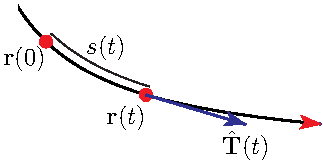
\includegraphics{fig/parCurveDerivB.pdf}}}
      \end{align*}
    \item 若以弧長為參數, 亦即 $t=s$ 使得 $\ds\diff{t}{s} = \diff{s}{s} = 1$, 則 $\ds\left|\diff{\vr}{s}(s)\right| = 1$, $\ds\widehat\vT(s) = \vr'(s)$. 
  \end{enumerate}
\end{prp}

\begin{prp} 給定位置向量 $\ds\vr(t)=\llt x(t)\,,\,y(t)\,,\,z(t)\rgt$, 則時點 $t$ 之
  \begin{itemize}\setlength{\itemsep}{0pt}
    \item 速度 $\ds\vv(t) = \vr'(t) = x'(t)\,\hi + y'(t)\,\hj + z'(t)\,\hk$
    \item 速率 $\ds\diff{s}{t}(t) = |\vv(t)| = |\vr'(t)| = \sqrt{(x'(t)^2 + y'(t)^2 + z'(t)^2}$
    \item 加速度 $\ds\va(t) = \vr''(t) = \vv'(t) = x''(t)\,\hi + y''(t)\,\hj + z''(t)\,\hk$
  \end{itemize}
  時點 $T_0$ 與 $T$ 間經過距離為 $\ds s(T)-s(T_0) = \int_{T_0}^T\Big|\diff{\vr}{t}(t)\Big|\,\dee{t} = \int_{T_0}^T\sqrt{(x'(t)^2+y'(t)^2+z'(t)^2}\,\dee{t}$
\end{prp}

\begin{ex}
  圓 $x^2+y^2=a^2$ 之曲線表示式為 $\ds\vr(\theta) = \llt a\cos\theta,\,a\sin\theta\rgt$, $0\leqslant\theta\leqslant 2\pi$. $\ds\vr'(\theta) = \llt-a\sin\theta,\,a\cos\theta\rgt$, $\ds\widehat\vT(\theta) = \frac{\vr'(\theta)}{|\vr'(\theta)|} = \llt-\sin\theta,\,\cos\theta\rgt$, $\ds\diff{s}{\theta}(\theta) = \big|\vr'(\theta)\big| = a$, $\ds s(\Theta) - s(0) = \int_{0}^\Theta\big|\vr'(\theta)\big|\,\dee{\theta} = a\Theta$. 
\end{ex}

\begin{figure}[!htbp]
  \centering
  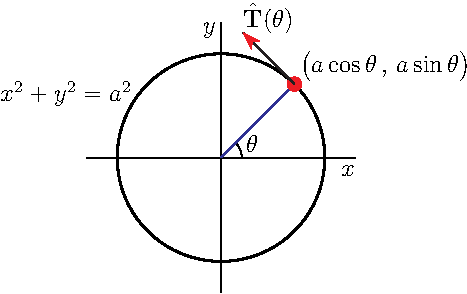
\includegraphics[scale=1]{fig/parCircleT.pdf}\qquad\qquad
  \raisebox{-20pt}[0pt][10pt]{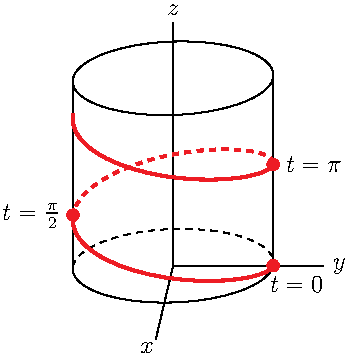
\includegraphics[scale=1]{fig/helix4.pdf}}
\end{figure}

\begin{ex}[螺旋線弧長]
  求 $\ds\vr(t) = 6\sin 2t\,\hi + 6\cos 2t\,\hj + 5t\,\hk$ 介於 $t = 0$ 與 $t = \pi$ 間弧長. 
\end{ex}
\begin{sol}
  $\ds\vr(t) = 6\sin 2t\,\hi + 6\cos 2t\,\hj + 5t\,\hk \ie \vr'(t) = 12\cos 2t\,\hi - 12\sin 2t\,\hj + 5\,\hk$. 則 $\ds\diff{s}{t}(t) = \big|\vr'(t)\big| = \sqrt{12^2\cos^2 2t + 12^2\sin^2 2t + 5^2} = \sqrt{12^2 + 5^2} = 13$, $\ds\widehat\vT(t) = \frac{\vr'(t)}{|\vr'(t)|} = \frac{12}{13}\cos 2t\;\hi -\frac{12}{13}\sin 2t\;\hj + \frac{5}{13}\,\hk$, \\$\ds s(\pi) - s(0) = \int_0^\pi\big|\vr'(t)\big|\,\dee{t} = 13\pi$. 
\end{sol}

\begin{ex}
  求 $\ds\vr(t) = \llt e^{3t},\,e^{-3t},\,3\sqrt{2}\,t\rgt$ 介於 $t = 0$ 與 $\ds t = \frac{1}{3}$ 間弧長. 
\end{ex}
\begin{sol}
  $\ds\vr'(t) = \llt 3e^{3t},\,-3e^{-3t},\,3\sqrt{2}\rgt$, $\ds s\Big(\frac{1}{3}\Big) - s(0) = \int_0^{\frac{1}{3}}\big|\vr'(t)\big|\,\dee{t} = \int_0^{\frac{1}{3}}\sqrt{9e^{6t} + 9e^{-6t} + 18}\,\dee{t} = 3\int_0^{\frac{1}{3}}\sqrt{e^{6t} + e^{-6t} + 2}\,\dee{t} \\= 3\int_0^{\frac{1}{3}}\sqrt{(e^{3t} + e^{-3t})^2}\,\dee{t} = 3\int_0^{\frac{1}{3}}(e^{3t} + e^{-3t})\,\dee{t} = e^{3t} - e^{-3t}\,\Big|_0^{\frac{1}{3}} = e - \frac{1}{e}$. 
\end{sol}

\begin{ex}
  求 $\ds\vr(t) = \llt t,\,2\,t,\,t^2\rgt$ 介於 $t = 1$ 與 $\ds t = 3$ 間弧長. 
\end{ex}
\begin{sol}
  $\ds\vr'(t) = \llt 1,\,2,\,2\,t\rgt$, $\ds s(3) - s(1) = \int_1^3\big|\vr'(t)\big|\,\dee{t} = \int_1^3\sqrt{5 + 4t^2}\,\dee{t} = \frac{6\sqrt{41} - 6 - 5\ln 5 + 5\ln(\sqrt{41} + 6)}{4}$, \\ 由 $\ds\int\!\sqrt{x^2 + a^2}\,\text{d}x = \frac{x\sqrt{x^2 + a^2} + a^2\ln\big|\sqrt{x^2 + a^2} + x\big|}{2} + c$. 
\end{sol}

\section*{5.3 極限與微分}

\begin{dfn}[多變數函數]
  令 $U\subseteq\mathbb{R}^n$, $n > 1$, 從 $U\to\mathbb{R}$ 的映射 $f(x_1,\,x_2,\,\ldots,\,x_n):U\to\mathbb{R}$ 稱為 $U$ 上的 $n$ 變數函數 (real-valued function of $n$ variables), 其中 $U$ 為定義域, $f(U)$ 為值域. 
\end{dfn}

\begin{rmk} 若 $f(x_1,\,x_2,\,\ldots,\,x_n)$ 為 $n$ 變數函數, 可將 $f$ 視為
  \begin{multicols}{2}
    \begin{itemize}\setlength{\itemsep}{0pt}
      \item $n$ 個實變數 $x_1,\,x_2,\,\ldots,\,x_n$ 的函數
      \item $\mathbb{R}^n$ 中之點 $(x_1,\,x_2,\,\ldots,\,x_n)$ 的函數
      \item 向量 $\vx = \llt x_1,\,x_2,\,\ldots,\,x_n\rgt$ 的函數
    \end{itemize}
  \end{multicols}
\end{rmk}

\begin{dfn}[圖形, 等值曲線]
  令 $f(x, y)$ 為定義在 $U$ 上的雙變數函數. 
  \begin{itemize}\setlength{\itemsep}{0pt}
    \item 集合 $\ds\left\{(x, y, z)\in\mathbb{R}^3\,|\,z = f(x, y),\;(x, y)\in U\right\}$ 稱為 $f$ 的圖形 (graph). 
    \item 給定常數 $k\in\mathbb{R}$, 曲線 $f(x, y) = k$ 稱為 $f$ 的等值曲線 (level / contour curve). 
  \end{itemize}
  若 $w = f(x, y, z)$ 為三變數函數, $f(x, y, z) = k$ 稱為 $f$ 的等值曲面 (level surface). 
\end{dfn}

\begin{dfn}[極限] 令 $f$ 為 $n$ 變數函數. 若對任意 $\varepsilon > 0$ 存在 $\delta > 0$ 使得對所有 $\vx\in\dom f$ 滿足 
  \begin{align*}
    0 < |\vx - \va| < \delta \ie |f(\vx) - L| < \varepsilon
  \end{align*}
  則稱 $f$ 在 $\va$ 的極限為 $L$, 記為 $\ds\lim_{\vx\to\va}f(\vx) = L$. 
\end{dfn}

\begin{prp}[極限運算]
  令 $\va\in\bbbr^n$, $c$, $F$, $G\in\bbbr$, $\ds D\subseteq\bbbr^n$, $f,\,g: D\setminus\{\va\}\to\bbbr$, $\ga:\bbbr\to\bbbr$.  
  %$\ds\vX:\bbbr^m\setminus\{\vb\}\to D\setminus\{\va\}$  $\ds\lim_{\vy\to\vb}\vX(\vy) = \va$
若 $\ds\lim_{\vx\to\va} f(\vx) = F$, $\ds\lim_{\vx\to\va} g(\vx) = G$, $\ds\lim_{t\to F}\ga(t) = \ga(F)$, 則
  \begin{multicols}{3}
    \begin{enumerate}\setlength{\itemsep}{0pt}
      \item $\ds\lim\limits_{\vx\to\va}\big[f(\vx)\pm g(\vx)\big] = F \pm G$
      \item $\ds\lim\limits_{\vx\to\va} f(\vx)\,g(\vx) = FG$
      \item $\ds\lim\limits_{\vx\to\va} \frac{f(\vx)}{g(\vx)} = \frac{F}{G}$ 若 $G\ne\vZero$
      %\item $\ds\lim\limits_{\vy\to \vb} f\big(\vX(\vy)\big) = F$
      \item $\ds\lim\limits_{\vx\to \va} \ga\big(f(\vx)\big) = \ga(F)$
    \end{enumerate}
  \end{multicols}
\end{prp}

\begin{ex} 
  求 $\ds\lim_{(x,\,y)\to(2,\,3)}\frac{x + \sin y}{x^2 y^2 + 1}$. 
\end{ex}

\begin{sol}
  $\ds\lim_{(x,\,y)\to (2,\,3)}\big(x + \sin y\big) = \lim_{(x,\,y)\to (2,\,3)}x + \lim_{(x,\,y)\to (2,\,3)}\sin y = \lim_{(x,\,y)\to (2,\,3)}x + \sin\left(\lim_{(x,\,y)\to (2,\,3)} y\right) = 2 + \sin 3$, $\ds\lim_{(x,\,y)\to (2,\,3)}\left(x^2 y^2 + 1\right) = \lim_{(x,\,y)\to (2,\,3)}x^2 y^2 + \lim_{(x,\,y)\to (2,\,3)}1 = \Big(\lim_{(x,\,y)\to (2,\,3)}x\Big)\Big(\lim_{(x,\,y)\to (2,\,3)}x\Big)\Big(\lim_{(x,\,y)\to (2,\,3)}y\Big)\Big(\lim_{(x,\,y)\to (2,\,3)}y\Big) + 1 = 2^2 3^2 + 1 = 37$, $\ds\lim_{(x,\,y)\to (2,\,3)}\frac{x + \sin y}{x^2 y^2 + 1} = \frac{\lim\limits_{(x,\,y)\to (2,\,3)}(x + \sin y)}{\lim\limits_{(x,\,y)\to (2,\,3)}(x^2 y^2 + 1)} = \frac{2 + \sin 3}{37}$
\end{sol}

\begin{rmk}
  \begin{itemize}\setlength{\itemsep}{0pt}
    \item[]
    \item 單變數函數極限 $\ds\lim_{x\to a} f(x)$ 存在的充要條件為 $\ds\lim_{x\to a-} f(x)$ 與 $\ds\lim_{x\to a+} f(x)$ 均存在且相等. 
    \item 多變數函數極限 $\ds\lim_{\vx\to\va} f(\vx)$ 存在的充要條件為{\color{M4}任意趨近 $\va$ 之路徑的極限}均存在且相等. 
    \item 求 $\ds\lim_{(x,\,y)\to(0,\,0)}f(x, y)$ 常可將 $(x,y)$ 轉成極座標 $\ds x = r\cos\theta$, $\ds y = r\sin\theta$ 後令 $r\to 0$ 觀察. 
  \end{itemize}

  %\begin{align*}
  %\hskip1in x&=r\cos\theta\hskip1in
  %\smash{\raisebox{-0.6\height}{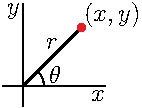
\includegraphics{fig/polar.pdf}}} \\
  %y&=r\sin\theta
  %\end{align*}
\end{rmk}

\begin{ex}
  求 $\ds\lim\limits_{(x,\,y)\to (0,\,0)}\frac{x^2y}{x^2+y^2}$. 
\end{ex}
\begin{sol}
  $\ds\frac{x^2y}{x^2+y^2} =\frac{(r\cos\theta)^2(r\sin\theta)}{r^2} = r\cos^2\theta\sin\theta$. 由 $\ds\big|r\cos^2\theta\sin\theta\big|\leqslant r\to 0$ 當 $r\to 0$, $\ds\lim\limits_{(x,\,y)\to (0,\,0)}\frac{x^2 y}{x^2 + y^2} = 0$. 
\end{sol}

\begin{ex}
  求 $\ds\lim\limits_{(x,\,y)\to (0,\,0)}\frac{x^2 - y^2}{x^2 + y^2}$. 
\end{ex}
\begin{sol}
  由 $\ds\frac{x^2 - y^2}{x^2 + y^2} = \frac{(r\cos\theta)^2 - (r\sin\theta)^2}{r^2} = \cos^2\theta - \sin^2\theta = \cos(2\theta)$, $\ds\lim\limits_{(x,\,y)\to (0,\,0)}\frac{x^2 - y^2}{x^2 + y^2} = \text{DNE}$
\end{sol}

\begin{ex}
  求 $\ds\lim\limits_{(x,\,y)\to (0,\,0)}\frac{2xy^2}{x^2+y^4}$. 
\end{ex}
\begin{sol}
  \begin{itemize}\setlength{\itemsep}{0pt}
    \item[]
    \item 令 $y = mx$, $m\ne 0$, 則 $\ds\lim_{(x,\,y)\to (0,\,0)}\frac{2xy^2}{x^2+y^4} = \lim_{x\to 0}\frac{2m^2x^3}{x^2 + m^4 x^4} = \lim_{x\to 0}\frac{2m^2x}{1 + m^4 x^2} = 0$. 
    \item 令 $x = y^2$, 則 $\ds\lim_{(x,\,y)\to (0,\,0)}\frac{2xy^2}{x^2+y^4} = \lim_{y\to 0}\frac{2y^4}{2y^4} = 1$. 
    \item 結論: $\ds\lim\limits_{(x,\,y)\to(0,\,0)}\frac{2xy^2}{x^2+y^4} = \text{DNE}$
  \end{itemize}
\end{sol}

\begin{ex}
  求 $\ds\lim\limits_{(x,\,y)\to (0,\,0)}\frac{x^2y^2}{x^2 + y^2}$. 
\end{ex}
\begin{sol}
  由 $\ds\frac{x^2y^2}{x^2 + y^2} = \frac{(r\cos\theta)^2(r\sin\theta)^2}{r^2} = r^2\cos^2\theta\sin^2\theta\leqslant\frac{r^2}{4}$, $\ds\lim\limits_{(x,\,y)\to (0,\,0)}\frac{x^2y^2}{x^2 + y^2} = 0$. 
\end{sol}

\begin{ex}
  求 $\ds\lim\limits_{(x,\,y)\to (0,\,0)}\frac{x^2y^2}{x^3 + y^3}$. 
\end{ex}
\begin{sol}
  \begin{itemize}\setlength{\itemsep}{0pt}
    \item[]
    \item 由 $\ds\frac{x^2y^2}{x^3 + y^3} = \frac{(r\cos\theta)^2(r\sin\theta)^2}{r^3(\cos^3\theta + \sin^3\theta)} = r\,\frac{\cos^2\theta\sin^2\theta}{\cos^3\theta + \sin^3\theta}$, 但 $\ds\frac{\cos^2\theta\sin^2\theta}{\cos^3\theta + \sin^3\theta}$ 非為有界 (取 $\ds\theta = \frac{3\pi}{4}$ 時 $\cos^3\theta + \sin^3\theta = 0$), $\ds\lim\limits_{(x,\,y)\to (0,\,0)}\frac{x^2y^2}{x^3 + y^3} = \lim_{r\to 0}\,r\,\frac{\cos^2\theta\sin^2\theta}{\cos^3\theta + \sin^3\theta} = \text{DNE}$. 
    \item 另解: 
      \begin{itemize}\setlength{\itemsep}{0pt}
        \item 令 $y = mx$, $m\ne 0$, 則 $\ds\lim_{(x,\,y)\to (0,\,0)}\frac{x^2y^2}{x^3 + y^3} = \lim_{x\to 0}\frac{x^2m^2x^2}{x^3 + m^3 x^3} = \lim_{x\to 0}\frac{m^2x}{1 + m^3} = 0$. 
        \item 令 $\ds y = -xe^x$, 則 $\ds\lim_{(x,\,y)\to (0,\,0)}\frac{x^2y^2}{x^3 + y^3} = \lim_{x\to 0}\frac{x^2x^2e^{2x}}{x^3 - x^3e^{3x}} = \lim_{x\to 0}\frac{xe^{2x}}{1 - e^{3x}} = \lim_{x\to 0}\frac{e^{2x}(1 + 2x)}{3e^{3x}} = \frac{1}{3}$. 
        \item 結論: $\ds\lim\limits_{(x,\,y)\to(0,\,0)}\frac{x^2y^2}{x^3 + y^3} = \text{DNE}$
      \end{itemize}
  \end{itemize}
\end{sol}

\begin{ex}
  求 $\ds\lim\limits_{(x,\,y)\to (0,\,0)}\frac{x^2y^2}{x^4 + y^4}$. 
\end{ex}
\begin{sol}
  \begin{itemize}\setlength{\itemsep}{0pt}
    \item[]
    \item 由 $\ds\frac{x^2y^2}{x^4 + y^4} = \frac{(r\cos\theta)^2(r\sin\theta)^2}{r^4(\cos^4\theta + \sin^4\theta)} = \frac{\cos^2\theta\sin^2\theta}{\cos^4\theta + \sin^4\theta}$, $\ds\lim\limits_{(x,\,y)\to (0,\,0)}\frac{x^2y^2}{x^4 + y^4} = \lim_{r\to 0}\frac{\cos^2\theta\sin^2\theta}{\cos^4\theta + \sin^4\theta} = \text{DNE}$. 
    \item 另解: 令 $y = mx$, $m\ne 0$, 則 $\ds\lim_{(x,\,y)\to (0,\,0)}\frac{x^2y^2}{x^4 + y^4} = \lim_{x\to 0}\frac{x^2m^2x^2}{x^4 + m^4 x^4} = \lim_{x\to 0}\frac{m^2}{1 + m^4} = \text{DNE}$. 
  \end{itemize}
\end{sol}

\begin{ex}
  若 $\ds f(x,y) = \begin{cases}\frac{(2x-y)^2}{x-y}, & x\ne y\\0, & x = y\end{cases}$, 求 $\ds\lim_{(x,\,y)\to (0,\,0)} f(x,y)$. 
\end{ex}
\begin{sol}
  \begin{itemize}\setlength{\itemsep}{0pt}
    \item[]
    \item 令 $y = x - x^3$, $\ds f(x,x - x^3) = \frac{{(2 x - x + x^3)}^2}{x - x + x^3} = \frac{{(x + x^3)}^2}{x^3} = \frac{{(1 + x^2)}^2}{x}\,\longrightarrow\,\begin{cases}+\infty, & x\to 0+\\-\infty, & x\to 0-\end{cases}$
    \item 令 $y = x - ax^2$, $a\ne 0$: $\ds\lim_{x\to 0}f(x,x - a x^2) = \lim_{x\to 0}\frac{{(2x - x + a x^2)}^2}{x - x + a x^2} = \lim_{x\to 0}\frac{{(x + a x^2)}^2}{a x^2} = \lim_{x\to 0}\frac{{(1 + a x)}^2}{a} = \frac{1}{a}$
    \item 結論: $\ds\lim\limits_{(x,\,y)\to(0,\,0)}f(x,y) = \text{DNE}$
  \end{itemize}
\end{sol}

\begin{dfn}[偏導函數, 偏微分, 偏導數]
  \begin{itemize}\setlength{\itemsep}{0pt}
    \item[]
    \item $\ds f(x, y)$ 的 $x$-偏導函數定義為 $\ds\pdiff{f}{x}(x, y) = \lim_{h\to 0}\frac{f(x + h, y) - f(x, y)}{h}$; $\ds f(x, y)$ 的 $y$-偏導函數定義為 $\ds\pdiff{f}{y}(x,y) = \lim_{h\to 0}\frac{f(x, y + h) - f(x, y)}{h}$. 
    \item 求 $f(x, y)$ 之 $x$-偏導函數之過程稱作「$\ds f(x, y)$ 對 $x$ 偏微分」. 
    \item $\ds f(x, y)$ 在 $(a, b)$ 的 $y$-偏導數記為 $\ds\pdiff{f}{y}(a,b)\equiv\pdiff{f}{y}\,\bigg|_{(a,b)}$. 
  \end{itemize}
\end{dfn}
\begin{rmk}
  \begin{itemize}\setlength{\itemsep}{0pt}
    \item[]
    \item $\ds\pdiff{f}{y}(x,y)$ 亦可記為 $\ds\pdiff{f}{y}$, $\ds f_y(x,y)$, $\ds f_y$, $\ds D_yf(x,y)$, $\ds D_yf$, $D_2 f(x,y)$, $D_2 f$. 
    \item 求 $\ds\pdiff{f}{y}(x, y)$:  將 $f(x, y)$ 中的 $x$ 視作常數, 然後對 $y$ 微分. 
    \item 求 $\ds\pdiff{f}{y}(a, b)$:  將 $f(x, y)$ 中的 $x$ 視作常數, 然後對 $y$ 微分並代入 $x = a$, $y = b$. 
    \item 以上符號 / 運算均可直接推廣至維度 $> 2$ 狀況. 
  \end{itemize}
\end{rmk}

\begin{ex}
  $\ds f(x,y) = x^3 + y^2 + 4xy^2$, 則 $\ds\pdiff{f}{x} = \pdiff{}{x}(x^3) + \pdiff{}{x}(y^2) + \pdiff{}{x}(4xy^2) = 3x^2 + 0 + 4y^2\pdiff{}{x}(x) = 3x^2 + 4y^2$, $\ds\pdiff{f}{y} = \pdiff{}{y}(x^3) + \pdiff{}{y}(y^2) +\pdiff{}{y}(4xy^2) = 0 + 2y + 4x\pdiff{}{y}(y^2) = 2y + 8xy$, $\ds\pdiff{f}{x}(1,\,0) = 3(1)^2 + 4(0)^2 = 3$, $\ds\pdiff{f}{y}(1,\,0) = 2(0) + 8(1)(0) = 0$. 
\end{ex}

\begin{ex}
  $\ds f(x,y) = y\cos x + xe^{xy}$, $\ds\pdiff{}{x} e^{yx}=y e^{yx}$, $\ds\pdiff{f}{x}(x,y) = y\pdiff{}{x}(\cos x) + e^{xy}\pdiff{}{x}(x) + x\pdiff{}{x}\big(e^{xy}\big) = -y\sin x + e^{xy} + x y e^{xy}$, $\ds\pdiff{f}{y}(x,y) = \cos x\pdiff{}{y}(y) + x\pdiff{}{y}\big(e^{xy}\big) = \cos x + x^2e^{xy}$
\end{ex}

\begin{ex}
  $\ds f(x, y, z, t) = x\sin(y + 2z) + t^2 e^{3y}\ln z$, 則 $\ds\pdiff{f}{x}(x,y,z,t) = \sin(y+2z)$, $\ds\pdiff{f}{y}(x,y,z,t) = x\cos(y+2z) +3t^2e^{3y}\ln z$, $\ds\pdiff{f}{z}(x,y,z,t) = 2x \cos(y + 2z) +\frac{t^2e^{3y}}{z}$, $\ds\pdiff{f}{t}(x,y,z,t) = 2t e^{3y}\ln z$. 
\end{ex}

\begin{ex} 若 $\ds f(x,y) = \begin{cases}\frac{\cos x - \cos y}{x - y} & x\ne y\\ 0 & x=y\end{cases}$
  \begin{itemize}\setlength{\itemsep}{0pt}
    \item $\forall\,x\ne y$, $\ds f_x = \frac{-\sin x(x - y) - (\cos x - \cos y)}{(x - y)^2}$; 無法由此求 $f_x(0, 0)$. 
    \item 由定義計算 $\ds f_x(0, 0)$: $\ds f_x(0, 0) = \lim_{h\to 0}\frac{f(0 + h, 0) - f(0, 0)}{h} = \lim_{h\to 0}\frac{\frac{\cos h - 1}{h - 0} - 0}{h} = \lim_{h\to 0}\frac{\cos h-1}{h^2} = \lim_{h\to 0}\frac{-\sin h}{2h} = \lim_{h\to 0}\frac{-\cos h}{2} = -\frac{1}{2}$. 
    \item 由定義計算 $\ds f_y(0, 0)$: $\ds f_y(0, 0) = \lim_{h\to 0}\frac{f(0, 0 + h) - f(0, 0)}{h} = \lim_{h\to 0}\frac{\frac{1 - \cos h}{-h} - 0}{h} = \lim_{h\to 0}\frac{\cos h-1}{h^2} = \lim_{h\to 0}\frac{-\sin h}{2h} = \lim_{h\to 0}\frac{-\cos h}{2} = -\frac{1}{2}$. 
    \item $\ds\lim_{(x,\,y)\to (0,\,0)}\frac{\cos x - \cos y}{x - y} = \lim_{(x,\,y)\to (0,\,0)}\frac{-2\sin\frac{x + y}{2}\sin\frac{x - y}{2}}{x - y} = -\lim_{(x,\,y)\to (0,\,0)}\sin\frac{x + y}{2}\,\lim_{(x,\,y)\to (0,\,0)}\frac{\sin\frac{x - y}{2}}{\frac{x - y}{2}} = 0$, 故 $f(x, y)$ 在 $(0, 0)$ 連續. 
    \item $\ds f(x, y)$ 在 $(a, a)$, $a\ne 0$ 不連續: 由定義 $\ds\lim_{(x,\,y)\to(a,\,a)}f(x, y) = \sin a$, 但 $f(a, a) = 0$. 
  \end{itemize}
\end{ex}

\begin{ex} 
  若 $x$, $y$, $z$ 滿足方程式 $\ds z^5 + y^2 e^z + e^{2x} = 0$, 求 $\ds\pdiff{z}{x}(0, 0)$. 
\end{ex}
\begin{sol}
  局域下 $z$ 為 $x$, $y$ 之函數; 當 $x = y = 0$, 原方程式為 $\ds z(0, 0)^5 = -1\ie z(0, 0) = -1$. 令 $z\equiv z(x, y)$ 代入原方程式並對 $x$ 偏微分得 $\ds 5\,z(x, y)^4\,\pdiff{z}{x}(x, y) + y^2\,e^{z(x, y)}\,\pdiff{z}{x}(x,y) + 2\,e^{2x} = 0$; 代入 $(x,\,y) = (0,\,0)$ 得 $\ds 5\,z(0, 0)^4\,\pdiff{z}{x}(0, 0) + 2  = 0$, 再由 $z(0, 0) = -1$, $\ds\pdiff{z}{x}(0, 0) = -\frac{2}{5\,z(0, 0)^4} = -\frac{2}{5}$. 
\end{sol}

\begin{ex}
  若 $x$, $y$, $z$ 滿足方程式 $\ds x^2 + y^2 + z^2 = 1$, 證明 $\ds x\,\pdiff{z}{x} + y\,\pdiff{z}{y} = z - \frac{1}{z}$. 
\end{ex}

\begin{sol}
  局域下 $z$ 為 $x$, $y$ 之函數; $\ds x^2 + y^2 + z^2 = 1$ 對 $x$ 偏微分得 $\ds 2x + 2z\,\pdiff{z}{x} = 0 \ie \pdiff{z}{x} = -\frac{x}{z}$; 對 $y$ 偏微分得 $\ds 2y + 2z\,\pdiff{z}{y} = 0 \ie \pdiff{z}{x} = -\frac{y}{z}$. 故 $\ds x\,\pdiff{z}{x} + y\,\pdiff{z}{y} = -\frac{x^2 + y^2}{z} = \frac{z^2 - 1}{z} = z - \frac{1}{z}$. 
\end{sol}

\begin{ex}
  若 $x$, $y$, $z$ 滿足方程式 $\ds x\sin z - z^2 y = 1$, 求 $\ds\pdiff{z}{x}$, $\ds\pdiff{z}{y}$. 
\end{ex}

\begin{sol}
  局域下 $z$ 為 $x$, $y$ 之函數; $\ds x\sin z - z^2 y = 1$ 對 $x$ 偏微分得 $\ds\sin z + x\cos z\,\pdiff{z}{x} - 2yz\,\pdiff{z}{x} = 0 \ie \pdiff{z}{x} = \frac{\sin z}{2yz - x\cos z}$; 對 $y$ 偏微分得 $\ds x\cos z\,\pdiff{z}{y} - 2z\,\pdiff{z}{y}\,y - z^2 = 0 \ie \pdiff{z}{y} = \frac{z^2}{x\cos z - 2yz}$. 
\end{sol}

\begin{dfn}[高階偏導函數] 給定可微雙變數函數 $f(x, y)$, 
  \begin{multicols}{2}
    \begin{itemize}\setlength{\itemsep}{0pt}
      \item $\ds\pdiff{}{x}\left(\pdiff{f}{x}\right)(x,y) = \frac{\partial^2 f}{\partial x^2}(x,y) = f_{xx}(x,y)$
      \item $\ds\pdiff{}{y}\left(\pdiff{f}{x}\right)(x,y) = \frac{\partial^2 f}{\partial y\partial x}(x,y) = f_{xy}(x,y)$
      \item $\ds\pdiff{}{x}\left(\pdiff{f}{y}\right)(x,y) = \frac{\partial^2 f}{\partial x\partial y}(x,y) = f_{yx}(x,y)$
      \item $\ds\pdiff{}{y}\left(\pdiff{f}{y}\right)(x,y) = \frac{\partial^2 f}{\partial y^2}(x,y) = f_{yy}(x,y)$
    \end{itemize}
  \end{multicols}
\end{dfn}

\begin{ex}
  令 $\ds f(x,y) = e^{my}\cos(nx)$, 則
  \begin{multicols}{3}
    \begin{itemize}\setlength{\itemsep}{0pt}
      \item $\ds f_x = -n e^{my}\sin(nx)$
      \item $\ds f_y = m e^{my}\cos(nx)$
      \item $\ds f_{xx} = -n^2 e^{my}\cos(nx)$
      \item $\ds f_{yy} = m^2 e^{my}\cos(nx)$
      \item $\ds f_{yx} = -m n e^{my}\sin(nx)$
      \item $\ds f_{xy} = -m n e^{my}\sin(nx)$
    \end{itemize}
  \end{multicols}
\end{ex}

\begin{ex}
  令 $\ds f(x,y) = e^{\al x+\be y}$, 則
  \begin{multicols}{3}
    \begin{itemize}\setlength{\itemsep}{0pt}
      \item $\ds f_x = \al e^{\al x+\be y}$ 
      \item $\ds f_y = \be e^{\al x+\be y}$
      \item $\ds f_{xx} = \al^2 e^{\al x+\be y}$
      \item $\ds f_{yx} = \be\al e^{\al x+\be y}$
      \item $\ds f_{xy} = \al\be e^{\al x+\be y}$
      \item $\ds f_{yy} = \be^2 e^{\al x+\be y}$
    \end{itemize}
  \end{multicols}
  對整數 $m, n\geqslant 0$, $\ds\frac{\partial^{m+n} f}{\partial x^m\partial y^n} = \al^m\be^n e^{\al x+\be y}$. 
\end{ex}

\begin{ex}
  令 $\ds f(x,y) = \ln(x^2 + y^2)$, 則
  \begin{multicols}{2}
    \begin{itemize}\setlength{\itemsep}{0pt}
      \item $\ds f_x = \frac{2x}{x^2 + y^2}$ 
      \item $\ds f_y = \frac{2y}{x^2 + y^2}$ 
      \item $\ds f_{xx} = \frac{(x^2 + y^2)\cdot 2 - 2x\cdot 2x}{(x^2 + y^2)^2} = \frac{2\,(y^2 - x^2)}{(x^2 + y^2)^2}$
      \item $\ds f_{yy} = \frac{(x^2 + y^2)\cdot 2 - 2y\cdot 2y}{(x^2 + y^2)^2} = \frac{2\,(x^2 - y^2)}{(x^2 + y^2)^2}$
    \end{itemize}
  \end{multicols}
  $\ds f(x, y)$ 滿足 Laplace 方程式 $\ds f_{xx} + f_{yy} = 0$. 
\end{ex}

\begin{ex}
  令 $\ds f(x,y) = \tan^{-1}\frac{y}{x}$, 則
  \begin{multicols}{2}
    \begin{itemize}\setlength{\itemsep}{0pt}
      \item $\ds f_x = \frac{1}{1 + \big(\frac{y}{x}\big)^2}\cdot\bigg(\frac{-y}{x^2}\bigg) = -\frac{y}{x^2 + y^2}$ 
      \item $\ds f_y = \frac{1}{1 + \big(\frac{y}{x}\big)^2}\cdot\bigg(\frac{1}{x}\bigg) = \frac{x}{x^2 + y^2}$ 
      \item $\ds f_{xx} = \frac{y\cdot 2x}{(x^2 + y^2)^2} = \frac{2 x y}{(x^2 + y^2)^2}$
      \item $\ds f_{yy} = -\frac{x\cdot 2y}{(x^2 + y^2)^2} = -\frac{2 x y}{(x^2 + y^2)^2}$
    \end{itemize}
  \end{multicols}
  $\ds f(x, y)$ 滿足 Laplace 方程式 $\ds f_{xx} + f_{yy} = 0$. 
\end{ex}

\begin{ex}
  若 $\ds f(x_1,x_2,x_3,x_4) = x_1^4\, x_2^3\, x_3^2\, x_4$, 則
  \begin{itemize}\setlength{\itemsep}{0pt}
    \item $\ds\frac{\partial^4 f}{\partial x_1\partial x_2\partial x_3\partial x_4} = \frac{\partial^3}{\partial x_1\partial x_2\partial x_3}\left(x_1^4 x_2^3 x_3^2\right) = \frac{\partial^2}{\partial x_1\partial x_2}\left(2 x_1^4 x_2^3 x_3\right) = \pdiff{}{x_1}\left(6 x_1^4 x_2^2 x_3\right) = 24 x_1^3 x_2^2 x_3$ 
    \item $\ds\frac{\partial^4 f}{\partial x_4\partial x_3\partial x_2\partial x_1} = \frac{\partial^3}{\partial x_4\partial x_3\partial x_2}\left(4 x_1^3 x_2^3 x_3^2 x_4\right) = \frac{\partial^2}{\partial x_4\partial x_3}\left(12 x_1^3 x_2^2 x_3^2 x_4\right) = \pdiff{}{x_4}\left(24 x_1^3 x_2^2 x_3 x_4\right) =  24 x_1^3 x_2^2 x_3$
  \end{itemize}
\end{ex}

\begin{thm}[Clairaut]
  若 $\ds\frac{\partial^2 f}{\partial x\partial y}$ 與 $\ds\frac{\partial^2 f}{\partial y\partial x}$ 均存在且在 $(x_0,\,y_0)$ 連續, 則 $\ds\frac{\partial^2 f}{\partial x\partial y}(x_0, y_0) = \frac{\partial^2 f}{\partial y\partial x}(x_0, y_0)$. 
\end{thm}

\section*{5.4 鏈鎖律} 
\begin{thm}
  若 $f$ 為 $x_1,\,x_2,\,\ldots,\,x_n$ 的可微函數, 而 $x_j$ 是 $t_1,\,t_2,\,\ldots,\,t_m$ 的可微函數, $n$, $m\geqslant 1$, 則 $f$ 為 $t_1,\,t_2,\,\ldots,\,t_m$ 的可微函數; 輔助函數 $F(t_1,\,t_2,\,\ldots,\,t_m)\equiv f(x_1(t_1,\,t_2,\,\ldots,\,t_m),\,x_2(t_1,\,t_2,\,\ldots,\,t_m),\,\ldots,\,x_n(t_1,\,t_2,\,\ldots,\,t_m))$, 則
  \begin{align*}
    \pdiff{F}{t_i} = \pdiff{f}{x_1}\,\pdiff{x_1}{t_i} + \pdiff{f}{x_2}\,\pdiff{x_2}{t_i} + \cdots + \pdiff{f}{x_n}\,\pdiff{x_n}{t_i}
  \end{align*}
\end{thm}

\begin{ex}[$n = m = 2$]
  輔助函數 $\ds F(s, t)\equiv f\big(x(s,t),\,y(s,t)\big)$, 則
  \begin{align*}
    \pdiff{F}{s}(s,t) &= \pdiff{f}{x}\big(x(s,t),\,y(s,t)\big)\,\pdiff{x}{s}(s,t) + \pdiff{f}{y}\big(x(s,t),\,y(s,t)\big)\,\pdiff{y}{s}(s,t) \\
    \pdiff{F}{t}(s,t) &= \pdiff{f}{x}\big(x(s,t),\,y(s,t)\big)\,\pdiff{x}{t}(s,t) + \pdiff{f}{y}\big(x(s,t),\,y(s,t)\big)\,\pdiff{y}{t}(s,t)
  \end{align*}
\end{ex}

\begin{ex}
  若 $\ds f(x, y) = e^{xy}$, $\ds x(s, t) = s$, $\ds y(s, t) = \cos t$; $\ds F(s, t)\equiv f\big(x(s,t),\,y(s,t)\big)$, 求 $\ds\pdiff{F}{s}$. 
\end{ex}
\begin{sol}
  \begin{itemize}\setlength{\itemsep}{0pt}
    \item[]
    \item $\ds\pdiff{f}{x} = y\,e^{xy} = y(s,t)\,e^{x(s,t)\,y(s,t)} = \cos t\,e^{s\cos t}$, $\ds\pdiff{f}{y} = x\,e^{xy} = x(s,t)\,e^{x(s,t)\,y(s,t)} = s\,e^{s\cos t}$, $\ds\pdiff{x}{s} = \pdiff{s}{s} = 1$, $\ds\pdiff{y}{s} = \pdiff{\cos t}{s} = 0$, 故 $\ds\pdiff{F}{s} = \pdiff{f}{x}\,\pdiff{x}{s} + \pdiff{f}{y}\,\pdiff{y}{s} = \cos t\,e^{s\cos t}\cdot 1 + s\ e^{s\cos t}\cdot 0 = \cos t\ e^{s\cos t}$. 
    \item 直接寫出 $F(s, t)$ 並對 $s$ 偏微分: $\ds F(s, t) = f\big(x(s,t),\,y(s,t)\big) = e^{s\cdot\cos t}$, $\ds\pdiff{F}{s} = e^{s\cdot\cos t}\,\cos t$.   
  \end{itemize}
\end{sol}

\begin{ex}
  若 $\ds f(x,y) = x^2 - y^2$, $x(t) = \cos t$, $y(t) = \sin t$, 求 $\ds\diff{f}{t}$. 
\end{ex}
\begin{sol}
  輔助函數 $\ds F(t)\equiv f\big(x(t),\,y(t)\big)$, 則
  \begin{itemize}\setlength{\itemsep}{0pt}
    \item $\ds\pdiff{f}{x} = 2x = 2\cos t$, $\ds\pdiff{f}{y} = -2y = -2\sin t$, $\ds\diff{x}{t} = -\sin t$, $\ds\diff{y}{t} = \cos t$, 故 $\ds\diff{F}{t} = \pdiff{f}{x}\,\diff{x}{t} + \pdiff{f}{y}\,\diff{y}{t} = (2\cos t)(-\sin t) + (-2\sin t)(\cos t) = -4\,\sin t\cos t$. 
    \item 直接寫出 $F(t)$ 並對 $t$ 微分: $\ds F(t) = f\big(x(t),y(t)\big) = x(t)^2 - y(t)^2 = \cos^2t - \sin^2t$, 故 $\ds F'(t) = 2(\cos t)(-\sin t)-2(\sin t)(\cos t) = -4 \sin t\cos t$
  \end{itemize}
\end{sol}

\begin{ex}
  \begin{enumerate}\setlength{\itemsep}{0pt}
    \item[]
    \item 令 $\ds w = xy + z$, $\ds x = \cos t$, $\ds y = \sin t$, $\ds z = t$, 求 $\ds\diff{w}{t}$ 與 $\ds\diff{w}{t}\Big|_{t = 0}$. 
    \item 令 $\ds w = x + 2y + z^2$, $\ds x = \frac{r}{s}$, $\ds y = r^2 + \ln s$, $\ds z = 2r$, 求 $\ds\pdiff{w}{r}$ 與 $\ds\pdiff{w}{s}$. 
    \item 令 $\ds w = x^4y + y^2z^3$, $\ds x = rse^{t}$, $\ds y = rs^2e^{-t}$, $\ds z = r^2s\sin t$, 求 $\ds\pdiff{w}{s}\Big|_{(r,\,s,\,t) = (2,\,1,\,0)}$. 
  \end{enumerate}
\end{ex}

\begin{sol}
  \begin{enumerate}\setlength{\itemsep}{0pt}
    \item[]
    \item $\ds\pdiff{w}{x} = y = \sin t$, $\ds\pdiff{w}{y} = x = \cos t$, $\ds\pdiff{w}{z} = 1$, $\ds\diff{x}{t} = -\sin t$, $\ds\diff{y}{t} = \cos t$, $\ds\diff{z}{t} = 1$, 故 $\ds\diff{w}{t} = \pdiff{w}{x}\,\diff{x}{t} + \pdiff{w}{y}\,\diff{y}{t} + \pdiff{w}{z}\,\diff{z}{t} = (\sin t)(-\sin t) + (\cos t)(\cos t) + (1)(1) = \cos 2t + 1$, $\ds\diff{w}{t}\Big|_{t = 0} = 1 + 1 = 2$. 
    \item $\ds\pdiff{w}{x} = 1$, $\ds\pdiff{w}{y} = 2$, $\ds\pdiff{w}{z} = 2 z = 4 r$, $\ds\pdiff{x}{r} = \frac{1}{s}$, $\ds\pdiff{y}{r} = 2r$, $\ds\pdiff{z}{r} = 2$, $\ds\pdiff{x}{s} = -\frac{r}{s^2}$, $\ds\pdiff{y}{s} = \frac{1}{s}$, $\ds\pdiff{z}{s} = 0$, 故 
      \begin{align*}
        \pdiff{w}{r} &= \pdiff{w}{x}\,\pdiff{x}{r} + \pdiff{w}{y}\,\pdiff{y}{r} + \pdiff{w}{z}\,\pdiff{z}{r} = (1)\Big(\frac{1}{s}\Big) + (2)(2r) + (4r)(2) = \frac{1}{s} + 12 r \\
        \pdiff{w}{s} &= \pdiff{w}{x}\,\pdiff{x}{s} + \pdiff{w}{y}\,\pdiff{y}{s} + \pdiff{w}{z}\,\pdiff{z}{s} = (1)\Big(-\frac{r}{s^2}\Big) + (2)\Big(\frac{1}{s}\Big) + (4r)(0) = -\frac{r}{s^2} + \frac{2}{s}
      \end{align*}
    %\item $\ds\pdiff{w}{x} = 4x^3y = 4(rse^{t})^3(rs^2e^{-t}) = 4 r^4s^5e^{2t}$, $\ds\pdiff{w}{y} = x^4 + 2yz^3 = r^4s^4e^{4t} + 2rs^2e^{-t}r^6s^3\sin^3 t = r^4s^4e^{4t} + 2r^7s^5e^{-t}\sin^3 t$, $\ds\pdiff{w}{z} = 3y^2z^2 = 3r^2s^4e^{-2t}\,r^4s^2\sin^2 t = 3r^6s^6e^{-2t}\sin^2 t$, $\ds\pdiff{x}{s} = re^{t}$, $\ds\pdiff{y}{s} = 2rse^{-t}$, $\ds\pdiff{z}{s} = r^2\sin t$, 故 $\ds\pdiff{w}{s}\Big|_{(r,\,s,\,t) = (2,\,1,\,0)} = \Big(\pdiff{w}{x}\,\pdiff{x}{s} + \pdiff{w}{y}\,\pdiff{y}{s} + \pdiff{w}{z}\,\pdiff{z}{s}\Big)\Big|_{(r,\,s,\,t) = (2,\,1,\,0)} = (4\cdot2^4\cdot1)(2) + (2^4\cdot1\cdot1)(2\cdot2\cdot1) + (0)(0) = 192$. 
    \item $\ds\pdiff{w}{x} = 4x^3y$, $\ds\pdiff{w}{y} = x^4 + 2yz^3$, $\ds\pdiff{w}{z} = 3y^2z^2$, $\ds\pdiff{x}{s} = re^{t}$, $\ds\pdiff{y}{s} = 2rse^{-t}$, $\ds\pdiff{z}{s} = r^2\sin t$. 當 $(r,\,s,\,t) = (2,\,1,\,0)$, $(x,\,y,\,z) = (2,\,2,\,0)$, 故
      \begin{align*}
        \pdiff{w}{s}\Big|_{(r,\,s,\,t) = (2,\,1,\,0)} &= \Big(\pdiff{w}{x}\,\pdiff{x}{s} + \pdiff{w}{y}\,\pdiff{y}{s} + \pdiff{w}{z}\,\pdiff{z}{s}\Big)\Big|_{(r,\,s,\,t) = (2,\,1,\,0)} \\ &= (4\cdot2^3\cdot2)(2) + (2^4 + 0)(2\cdot2\cdot1) + (0)(0) = 192
      \end{align*}
  \end{enumerate}
\end{sol}

\begin{ex}
  若 $\ds z = f(x - y)$, 證明 $\ds\pdiff{z}{x} + \pdiff{z}{y} = 0$. 
\end{ex}

\begin{sol} 令 $\ds u = x - y$, 則 $\ds\pdiff{z}{x} = \diff{z}{u}\,\pdiff{u}{x} = \diff{z}{u}(1) = \diff{z}{u}$, $\ds\pdiff{z}{y} = \diff{z}{u}\,\pdiff{u}{y} = \diff{z}{u}(-1) = -\diff{z}{u}$, 故 $\ds\pdiff{z}{x} + \pdiff{z}{y} = 0$. 
\end{sol}

\begin{ex}
  若 $\ds z = f(x, y)$, $\ds x = s + t$, $\ds y = s - t$, 證明 $\ds\bigg(\pdiff{z}{x}\bigg)^2 - \bigg(\pdiff{z}{y}\bigg)^2 = \pdiff{z}{s}\pdiff{z}{t}$. 
\end{ex}

\begin{sol} 
  $\ds\pdiff{z}{s} = \pdiff{z}{x}\,\pdiff{x}{s} + \pdiff{z}{y}\,\pdiff{y}{s} = \pdiff{z}{x} + \pdiff{z}{y}$, $\ds\pdiff{z}{t} = \pdiff{z}{x}\,\pdiff{x}{t} + \pdiff{z}{y}\,\pdiff{y}{t} = \pdiff{z}{x} - \pdiff{z}{y}$, 故 $\ds\pdiff{z}{s}\,\pdiff{z}{t} = \bigg(\pdiff{z}{x}\bigg)^2 - \bigg(\pdiff{z}{y}\bigg)^2$. 
\end{sol}

\begin{ex}
  若 $\ds g(s, t) = f(s^2 - t^2, t^2 - s^2)$ 且 $f$ 可微, 證明 $\ds t\,\pdiff{g}{s} + s\,\pdiff{g}{t} = 0$. 
\end{ex}

\begin{sol}
  令 $\ds u(s, t) = s^2 - t^2$, $\ds v(s, t) = t^2 - s^2$, 則 $\ds g(s, t) = f(u(s, t), v(s, t))$. 由鏈鎖律 
  \begin{align*}
    \pdiff{g}{s} &= \pdiff{f}{u}\,\pdiff{u}{s} + \pdiff{f}{v}\,\pdiff{v}{s} = \pdiff{f}{u}\cdot(2s) + \pdiff{f}{v}\cdot(-2s) \\
    \pdiff{g}{t} &= \pdiff{f}{u}\,\pdiff{u}{t} + \pdiff{f}{v}\,\pdiff{v}{t} = \pdiff{f}{u}\cdot(-2t) + \pdiff{f}{v}\cdot(2t)
  \end{align*}
  故 $\ds t\,\pdiff{g}{s} + s\,\pdiff{g}{t} = t\,\bigg(\pdiff{f}{u}\cdot(2s) + \pdiff{f}{v}\cdot(-2s)\bigg) + s\,\bigg(\pdiff{f}{u}\cdot(-2t) + \pdiff{f}{v}\cdot(2t)\bigg) = 0$.  
\end{sol}

\begin{ex}
  若函數 $f(x, y)$ 滿足 $\ds f(tx, ty) = t^n f(x, y)$, $t\ne 0$, $n\in\mathbb{N}$, 稱 $f(x, y)$ 為 $n$ 次齊次函數% (homogeneous of degree $n$)
; 證明
  \begin{multicols}{2}
    \begin{enumerate}\setlength{\itemsep}{0pt}
      \item $\ds x\pdiff{f}{x} + y\pdiff{f}{y} = nf$.
      \item $\ds x^2\pdifft{f}{x} + 2xy\frac{\partial^2 f}{\partial x\partial y} + y^2\pdifft{f}{y} = n(n - 1)f$.
    \end{enumerate}
  \end{multicols}
\end{ex}

\begin{sol}
  令 $u(x, y, t) = tx$, $v(x, y, t) = ty$, 則 $\ds f(u(x, y, t), v(x, y, t)) = t^n f(x, y)$. 
  \begin{enumerate}\setlength{\itemsep}{0pt}
    \item 等式 $\ds f(u(x, y, t), v(x, y, t)) = t^n f(x, y)$ 兩邊對 $t$ 微分 $\ie$ $\ds\pdiff{f}{u}(tx, ty)\pdiff{u}{t} + \pdiff{f}{v}(tx, ty)\pdiff{v}{t} = n t^{n - 1}f(x, y)$ $\ie$ $\ds x\pdiff{f}{u}(tx, ty) + y\pdiff{f}{v}(tx, ty) = n t^{n - 1}f(x, y)$. 令 $t = 1$ 則 $\ds x\pdiff{f}{x} + y\pdiff{f}{y} = nf$.
    \item 等式 $\ds x\pdiff{f}{u}(tx, ty) + y\pdiff{f}{v}(tx, ty) = n t^{n - 1}f(x, y)$ 兩邊對 $t$ 微分 $\ie$ $\ds\pdiff{}{t}\bigg(x\pdiff{f}{u}(tx, ty) + y\pdiff{f}{v}(tx, ty)\bigg) = n(n - 1) t^{n - 2}f(x, y)$ $\ie$ $\ds x\pdiff{}{t}\bigg(\pdiff{f}{u}(tx, ty)\bigg) + y\pdiff{}{t}\bigg(\pdiff{f}{v}(tx, ty)\bigg) = n(n - 1) t^{n - 2}f(x, y)$. 又 $\ds\pdiff{}{t}\bigg(\pdiff{f}{u}(tx, ty)\bigg)$ $=$ $\ds\pdifft{f}{u}(tx, ty)\pdiff{u}{t} + \frac{\partial^2 f}{\partial v\partial u}(tx, ty)\pdiff{v}{t}$ $=$ $\ds x\pdifft{f}{u}(tx, ty) + y\frac{\partial^2 f}{\partial v\partial u}(tx, ty)$, $\ds\pdiff{}{t}\bigg(\pdiff{f}{v}(tx, ty)\bigg)$ $=$ $\ds\frac{\partial^2 f}{\partial u\partial v}(tx, ty)\pdiff{u}{t} + \pdifft{f}{v}(tx, ty)\pdiff{v}{t}$ $=$ $\ds x\frac{\partial^2 f}{\partial u\partial v}(tx, ty) + y\pdifft{f}{v}(tx, ty)$, 故 $\ds x\pdiff{}{t}\bigg(\pdiff{f}{u}(tx, ty)\bigg) + y\pdiff{}{t}\bigg(\pdiff{f}{v}(tx, ty)\bigg) = x^2\pdifft{f}{u}(tx, ty) + xy\frac{\partial^2 f}{\partial v\partial u}(tx, ty) + yx\frac{\partial^2 f}{\partial u\partial v}(tx, ty) + y^2\pdifft{f}{v}(tx, ty) = n(n - 1) t^{n - 2}f(x, y)$; 令 $t = 1$ 則 $\ds x^2\pdifft{f}{x} + 2xy\frac{\partial^2 f}{\partial x\partial y} + y^2\pdifft{f}{y} = n(n - 1)f$.
  \end{enumerate}
\end{sol}

\begin{ex}
  若 $\ds u = f(x, y)$, $\ds x = e^s\cos t$, $\ds y = e^s\sin t$, 證明 $\ds\bigg(\pdiff{u}{x}\bigg)^2 + \bigg(\pdiff{u}{y}\bigg)^2 = e^{-2s}\bigg(\bigg(\pdiff{u}{s}\bigg)^2 + \bigg(\pdiff{u}{t}\bigg)^2\bigg)$.   
\end{ex}

\begin{sol} 由鏈鎖律
  \begin{align*}
    \pdiff{u}{s} &= \pdiff{u}{x}\,\pdiff{x}{s} + \pdiff{u}{y}\,\pdiff{y}{s} = \pdiff{u}{x}\cdot(e^s\cos t) + \pdiff{u}{y}\cdot(e^s\sin t)\\
    \pdiff{u}{t} &= \pdiff{u}{x}\,\pdiff{x}{t} + \pdiff{u}{y}\,\pdiff{y}{t} = \pdiff{u}{x}\cdot(-e^s\sin t) + \pdiff{u}{y}\cdot(e^s\cos t)
  \end{align*}
  故
  \begin{align*}
    \bigg(\pdiff{u}{s}\bigg)^2 + \bigg(\pdiff{u}{t}\bigg)^2 &= \bigg(\pdiff{u}{x}\cdot(e^s\cos t) + \pdiff{u}{y}\cdot(e^s\sin t)\bigg)^2 + \bigg(\pdiff{u}{x}\cdot(-e^s\sin t) + \pdiff{u}{y}\cdot(e^s\cos t)\bigg)^2 \\
    &= \bigg(\pdiff{u}{x}\bigg)^2 e^{2s} \cos^2 t + 2\,\pdiff{u}{x}\pdiff{u}{y}e^{2s}\cos t\sin t + \bigg(\pdiff{u}{y}\bigg)^2 e^{2s}\sin^2 t \\ &\; + \bigg(\pdiff{u}{x}\bigg)^2 e^{2s}\sin^2 t - 2\,\pdiff{u}{x}\pdiff{u}{y} e^{2s} \sin t\cos t + \bigg(\pdiff{u}{y}\bigg)^2 e^{2s} cos^2 t = e^{2s}\bigg(\bigg(\pdiff{u}{x}\bigg)^2 + \bigg(\pdiff{u}{y}\bigg)^2\bigg) 
  \end{align*}
\end{sol}

\begin{ex}
  若 $\ds z = f(x, y)$, $\ds x = r\cos\theta$, $\ds y = r\sin\theta$, 證明 $\ds\bigg(\pdiff{z}{x}\bigg)^2 + \bigg(\pdiff{z}{y}\bigg)^2 = \bigg(\pdiff{z}{r}\bigg)^2 + \frac{1}{r^2}\,\bigg(\pdiff{z}{\theta}\bigg)^2$.   
\end{ex}

\begin{sol} 由鏈鎖律
  \begin{align*}
    \pdiff{z}{r} &= \pdiff{z}{x}\,\pdiff{x}{r} + \pdiff{z}{y}\,\pdiff{y}{r} = \pdiff{z}{x}\cos\theta + \pdiff{z}{y}\sin\theta \\
    \pdiff{z}{\theta} &= \pdiff{z}{x}\,\pdiff{x}{\theta} + \pdiff{z}{y}\,\pdiff{y}{\theta} = \pdiff{z}{x}\cdot(-r\sin\theta) + \pdiff{z}{y}\cdot(r\cos\theta)
  \end{align*}
  故
  \begin{align*}
    \bigg(\pdiff{z}{r}\bigg)^2 + \frac{1}{r^2}\,\bigg(\pdiff{z}{\theta}\bigg)^2 &= \bigg(\pdiff{z}{x}\cos\theta + \pdiff{z}{y}\sin\theta\bigg)^2 + \frac{1}{r^2}\,\bigg(\pdiff{z}{x}\cdot(-r\sin\theta) + \pdiff{z}{y}\cdot(r\cos\theta)\bigg)^2 \\
    &= \bigg(\pdiff{z}{x}\bigg)^2\cos^2\theta + 2\,\pdiff{z}{x}\pdiff{z}{y}\cos\theta\sin\theta + \bigg(\pdiff{z}{y}\bigg)^2\sin^2\theta \\ &\; + \bigg(\pdiff{z}{x}\bigg)^2\sin^2\theta - 2\,\pdiff{z}{x}\pdiff{z}{y}\sin\theta\cos\theta + \bigg(\pdiff{z}{y}\bigg)^2\cos^2\theta = \bigg(\pdiff{z}{x}\bigg)^2 + \bigg(\pdiff{z}{y}\bigg)^2 
  \end{align*}
\end{sol}
\begin{ex}
  若 $\ds z = u(x, y)$, $\ds x = r^2 + s^2$, $\ds y = 2rs$, 求 $\ds\pdiff{z}{r}$, $\ds\pdifft{z}{r}$, $\ds\frac{\partial^2 z}{\partial s\partial r}$. 
\end{ex}

\begin{sol} 由鏈鎖律
  \begin{align*}
    \pdiff{z}{r} &= \pdiff{u}{x}\,\pdiff{x}{r} + \pdiff{u}{y}\,\pdiff{y}{r} = 2r\,\pdiff{u}{x} + 2s\,\pdiff{u}{y} \\
    \pdifft{z}{r} &= \pdiff{}{r}\left(2r\,\pdiff{u}{x} + 2s\,\pdiff{u}{y}\right) = 2\,\pdiff{u}{x} + 2r\,\pdiff{}{r}\bigg(\pdiff{u}{x}\bigg) + 2s\,\pdiff{}{r}\bigg(\pdiff{u}{y}\bigg) \\ 
    \frac{\partial^2 z}{\partial s\partial r} &= \pdiff{}{s}\left(2r\,\pdiff{u}{x} + 2s\,\pdiff{u}{y}\right) = 2\,\pdiff{u}{y} + 2s\,\pdiff{}{s}\bigg(\pdiff{u}{y}\bigg) + 2r\,\pdiff{}{s}\bigg(\pdiff{u}{x}\bigg) 
  \end{align*}
  又
  \begin{align*}
    \pdiff{}{r}\bigg(\pdiff{u}{x}\bigg) &= \pdiff{}{x}\bigg(\pdiff{u}{x}\bigg)\,\pdiff{x}{r} + \pdiff{}{y}\bigg(\pdiff{u}{x}\bigg)\,\pdiff{y}{r} = \pdifft{u}{x}\cdot(2r) + \frac{\partial^2 u}{\partial y\partial x}\cdot(2s) \\
    \pdiff{}{r}\bigg(\pdiff{u}{y}\bigg) &= \pdiff{}{x}\bigg(\pdiff{u}{y}\bigg)\,\pdiff{x}{r} + \pdiff{}{y}\bigg(\pdiff{u}{y}\bigg)\,\pdiff{y}{r} = \frac{\partial^2 u}{\partial x\partial y}\cdot(2r) + \pdifft{u}{y}\cdot(2s) \\
    \pdiff{}{s}\bigg(\pdiff{u}{x}\bigg) &= \pdiff{}{x}\bigg(\pdiff{u}{x}\bigg)\,\pdiff{x}{s} + \pdiff{}{y}\bigg(\pdiff{u}{x}\bigg)\,\pdiff{y}{s} = \pdifft{u}{x}\cdot(2s) + \frac{\partial^2 u}{\partial y\partial x}\cdot(2r) \\
    \pdiff{}{s}\bigg(\pdiff{u}{y}\bigg) &= \pdiff{}{x}\bigg(\pdiff{u}{y}\bigg)\,\pdiff{x}{s} + \pdiff{}{y}\bigg(\pdiff{u}{y}\bigg)\,\pdiff{y}{s} = \frac{\partial^2 u}{\partial x\partial y}\cdot(2s) + \pdifft{u}{y}\cdot(2r)
  \end{align*}
  故
  \begin{align*}
    \pdifft{z}{r} &= 2\,\pdiff{u}{x} + 2r\,\pdiff{}{r}\bigg(\pdiff{u}{x}\bigg) + 2s\,\pdiff{}{r}\bigg(\pdiff{u}{y}\bigg) \\
    &= 2\,\pdiff{u}{x} + 2r\,\bigg(\pdifft{u}{x}\cdot(2r) + \frac{\partial^2 u}{\partial y\partial x}\cdot(2s)\bigg) + 2s\,\bigg(\frac{\partial^2 u}{\partial x\partial y}\cdot(2r) + \pdifft{u}{y}\cdot(2s)\bigg) \\
    &= 2\,\pdiff{u}{x} + 4r^2\,\pdifft{u}{x} + 8rs\,\frac{\partial^2 u}{\partial x\partial y} + 4s^2\,\pdifft{u}{y} \\
    \frac{\partial^2 z}{\partial s\partial r} &= 2\,\pdiff{u}{y} + 2s\,\pdiff{}{s}\bigg(\pdiff{u}{y}\bigg) + 2r\,\pdiff{}{s}\bigg(\pdiff{u}{x}\bigg) \\
    &= 2\,\pdiff{u}{y} + 2s\,\bigg(\frac{\partial^2 u}{\partial x\partial y}\cdot(2s) + \pdifft{u}{y}\cdot(2r)\bigg) + 2r\,\bigg(\pdifft{u}{x}\cdot(2s) + \frac{\partial^2 u}{\partial y\partial x}\cdot(2r)\bigg) \\
    &= 2\,\pdiff{u}{y} + 4rs\,\pdifft{u}{x} + 4(r^2 + s^2)\,\frac{\partial^2 u}{\partial x\partial y} + 4rs\,\pdifft{u}{y}
  \end{align*}
\end{sol}

\begin{ex}
  若 $\ds z = u(x, y)$, $\ds x = g(s, t)$, $\ds y = h(s, t)$, 證明 
  \begin{align*}
    \pdifft{z}{t} = \pdiff{z}{x}\pdifft{x}{t} + \pdiff{z}{y}\pdifft{y}{t} + \pdifft{z}{x}\bigg(\pdiff{x}{t}\bigg)^2 + 2\,\frac{\partial^2 z}{\partial x\partial y}\pdiff{x}{t}\pdiff{y}{t} + \pdifft{z}{y}\bigg(\pdiff{y}{t}\bigg)^2
  \end{align*}
\end{ex}

\begin{sol}
  令 $\ds z = U(s, t) = u(x(s, t),\,y(s, t))$, 由鏈鎖律 
  \begin{align*}
    \pdiff{U}{t} &= \pdiff{u}{x}\,\pdiff{x}{t} + \pdiff{u}{y}\,\pdiff{y}{t} \\
    \pdifft{U}{t} &= \pdiff{}{t}\bigg(\pdiff{u}{x}\,\pdiff{x}{t} + \pdiff{u}{y}\,\pdiff{y}{t}\bigg) = \pdiff{u}{x}\pdifft{x}{t} + \pdiff{x}{t}\pdiff{}{t}\bigg(\pdiff{u}{x}\bigg) + \pdiff{u}{y}\pdifft{y}{t} + \pdiff{y}{t}\pdiff{}{t}\bigg(\pdiff{u}{y}\bigg) 
  \end{align*}
  又
  \begin{align*}
    \pdiff{}{t}\bigg(\pdiff{u}{x}\bigg) &= \pdiff{}{x}\left(\pdiff{u}{x}\right)\,\pdiff{x}{t} + \pdiff{}{y}\bigg(\pdiff{u}{x}\bigg)\,\pdiff{y}{t} = \pdifft{u}{x}\,\pdiff{x}{t} + \frac{\partial^2 u}{\partial y\partial x}\,\pdiff{y}{t}\\
    \pdiff{}{t}\bigg(\pdiff{u}{y}\bigg) &= \pdiff{}{x}\left(\pdiff{u}{y}\right)\,\pdiff{x}{t} + \pdiff{}{y}\bigg(\pdiff{u}{y}\bigg)\,\pdiff{y}{t} = \frac{\partial^2 u}{\partial x\partial y}\,\pdiff{x}{t} + \pdifft{u}{y}\,\pdiff{y}{t}
  \end{align*}
  故
  \begin{align*}
    \pdifft{U}{t} &= \pdiff{u}{x}\pdifft{x}{t} + \pdiff{x}{t}\left(\pdifft{u}{x}\,\pdiff{x}{t} + \pdiff{u}{y}\pdifft{y}{t} + \frac{\partial^2 u}{\partial y\partial x}\,\pdiff{y}{t}\right) + \pdiff{y}{t}\left(\frac{\partial^2 u}{\partial x\partial y}\,\pdiff{x}{t} + \pdifft{u}{y}\,\pdiff{y}{t}\right) \\ &= \pdiff{u}{x}\pdifft{x}{t} + \pdiff{u}{y}\pdifft{y}{t} + \pdifft{u}{x}\bigg(\pdiff{x}{t}\bigg)^2 + 2\,\frac{\partial^2 u}{\partial x\partial y}\,\pdiff{x}{t}\pdiff{y}{t} + \pdifft{u}{y}\bigg(\pdiff{y}{t}\bigg)^2
  \end{align*}
\end{sol}

\begin{ex} 若 $\ds f(x, t) = g(x + at) + h(x - at)$, 其中 $g$, $h$ 可二次微分, 證明 $f$ 滿足波動方程式 $\ds\pdifft{f}{t} = a^2\pdifft{f}{x}$. 
\end{ex}

\begin{sol}
  令 $\ds u(x, t) = x + at$, $\ds v(x, t) = x - at$, $\ds f\big(u(x,t), v(x, t)\big) = g(u(x, t)) + h(v(x, t))$. 由鏈鎖律 
  \begin{align*}
    \pdiff{f}{t} &= \pdiff{f}{u}\,\pdiff{u}{t} + \pdiff{f}{v}\,\pdiff{v}{t} \\
                 &= g'(u(x, t))\cdot a + h'(v(x, t))\cdot(-a) = a\,g'(x + at) - a\,h'(x - at) = a\,g'(u(x, t)) - a\,h'(v(x, t)) \\
    \pdifft{f}{t} &= \pdiff{}{t}\bigg(\pdiff{f}{t}\bigg) \\ 
    &= \pdiff{}{u}\big(a\,g'(u) - a\,h'(v)\big)\big(u(x,t), v(x, t)\big)\,\pdiff{u}{t} + \pdiff{}{v}\big(a\,g'(u) - a\,h'(v)\big)\big(u(x,t), v(x, t)\big)\pdiff{v}{t} \\ &= a\,g''(u(x,t))\cdot a - a\,h''(v(x, t))\cdot(-a) \\ &= a^2\,(g''(x + at) + h''(x - at)) \\
    \pdiff{f}{x} &= \pdiff{f}{u}\,\pdiff{u}{x} + \pdiff{f}{v}\,\pdiff{v}{x} \\
                 &= g'(u(x, t))\cdot 1 + h'(v(x, t))\cdot(1) = g'(x + at) + h'(x - at) = g'(u(x, t)) + h'(v(x, t)) \\
    \pdifft{f}{x} &= \pdiff{}{x}\bigg(\pdiff{f}{x}\bigg) \\ 
    &= \pdiff{}{x}\big(g'(u) + h'(v)\big)\big(u(x,t), v(x, t)\big)\,\pdiff{u}{x} + \pdiff{}{v}\big(g'(u) + h'(v)\big)\big(u(x,t), v(x, t)\big)\pdiff{v}{x} \\ 
    &= g''(u(x,t))\cdot 1 + h''(v(x, t))\cdot 1\\ 
    &= g''(x + at) + h''(x - at)
  \end{align*}
  故 $\ds\pdifft{f}{t} = a^2\pdifft{f}{x}$. 
\end{sol}

\begin{ex}
  若 $\ds u = f(x, y)$, $\ds x = e^s\cos t$, $\ds y = e^s\sin t$, 證明 $\ds\pdifft{u}{x} + \pdifft{u}{y} = e^{-2s}\bigg(\pdifft{u}{s} + \pdifft{u}{t}\bigg)$.   
\end{ex}

\begin{sol} 由鏈鎖律
  \begin{align*}
    \pdiff{u}{s} &= \pdiff{u}{x}\,\pdiff{x}{s} + \pdiff{u}{y}\,\pdiff{y}{s} = \pdiff{u}{x}\cdot(e^s\cos t) + \pdiff{u}{y}\cdot(e^s\sin t)\\
    \pdiff{u}{t} &= \pdiff{u}{x}\,\pdiff{x}{t} + \pdiff{u}{y}\,\pdiff{y}{t} = \pdiff{u}{x}\cdot(-e^s\sin t) + \pdiff{u}{y}\cdot(e^s\cos t) 
  \end{align*}

  \begin{align*}
    \pdifft{u}{s} = \pdiff{}{s}\bigg(\pdiff{u}{s}\bigg) &= \pdiff{}{s}\bigg(\pdiff{u}{x}\cdot(e^s\cos t) + \pdiff{u}{y}\cdot(e^s\sin t)\bigg)\\
    &= \pdiff{}{s}\bigg(\pdiff{u}{x}\bigg)\cdot(e^s\cos t) + \pdiff{u}{x}\cdot(e^s\cos t) + \pdiff{}{s}\bigg(\pdiff{u}{y}\bigg)\cdot(e^s\sin t) + \pdiff{u}{y}\cdot(e^s\sin t) \\
    \pdifft{u}{t} = \pdiff{}{t}\bigg(\pdiff{u}{t}\bigg) &= \pdiff{}{t}\bigg(\pdiff{u}{x}\cdot(-e^s\sin t) + \pdiff{u}{y}\cdot(e^s\cos t)\bigg)\\
    &= \pdiff{}{t}\bigg(\pdiff{u}{x}\bigg)\cdot(-e^s\sin t) + \pdiff{u}{x}\cdot(-e^s\cos t) + \pdiff{}{t}\bigg(\pdiff{u}{y}\bigg)\cdot(e^s\cos t) + \pdiff{u}{y}\cdot(-e^s\sin t)
  \end{align*}
  又
  \begin{align*}
    \pdiff{}{s}\bigg(\pdiff{u}{x}\bigg) &= \pdiff{}{x}\left(\pdiff{u}{x}\right)\,\pdiff{x}{s} + \pdiff{}{y}\bigg(\pdiff{u}{x}\bigg)\,\pdiff{y}{s} = \pdifft{u}{x}\cdot(e^s\cos t) + \frac{\partial^2 u}{\partial y\partial x}\cdot(e^s\sin t)\\
  \pdiff{}{s}\bigg(\pdiff{u}{y}\bigg) &= \pdiff{}{x}\left(\pdiff{u}{y}\right)\,\pdiff{x}{s} + \pdiff{}{y}\bigg(\pdiff{u}{y}\bigg)\,\pdiff{y}{s} = \frac{\partial^2 u}{\partial x\partial y}\cdot(e^s\cos t) + \pdifft{u}{y}\cdot(e^s\sin t) \\
    \pdiff{}{t}\bigg(\pdiff{u}{x}\bigg) &= \pdiff{}{x}\left(\pdiff{u}{x}\right)\,\pdiff{x}{t} + \pdiff{}{y}\bigg(\pdiff{u}{x}\bigg)\,\pdiff{y}{t} = \pdifft{u}{x}\cdot(-e^s\sin t) + \frac{\partial^2 u}{\partial y\partial x}\cdot(e^s\cos t)\\
  \pdiff{}{t}\bigg(\pdiff{u}{y}\bigg) &= \pdiff{}{x}\left(\pdiff{u}{y}\right)\,\pdiff{x}{t} + \pdiff{}{y}\bigg(\pdiff{u}{y}\bigg)\,\pdiff{y}{t} = \frac{\partial^2 u}{\partial x\partial y}\cdot(-e^s\sin t) + \pdifft{u}{y}\cdot(e^s\cos t)
  \end{align*}
  故
  \begin{align*}
    \pdifft{u}{s} &= \pdiff{}{s}\bigg(\pdiff{u}{x}\bigg)\cdot(e^s\cos t) + \pdiff{u}{x}\cdot(e^s\cos t) + \pdiff{}{s}\bigg(\pdiff{u}{y}\bigg)\cdot(e^s\sin t) + \pdiff{u}{y}\cdot(e^s\sin t) \\
    &= \bigg(\pdifft{u}{x}\cdot(e^s\cos t) + \frac{\partial^2 u}{\partial y\partial x}\cdot(e^s\sin t)\bigg)\cdot(e^s\cos t) + \pdiff{u}{x}\cdot(e^s\cos t)\\
    &\;+ \bigg(\frac{\partial^2 u}{\partial x\partial y}\cdot(e^s\cos t) + \pdifft{u}{y}\cdot(e^s\sin t)\bigg)\cdot(e^s\sin t) + \pdiff{u}{y}\cdot(e^s\sin t)\\
    \pdifft{u}{t} &= \pdiff{}{t}\bigg(\pdiff{u}{x}\bigg)\cdot(-e^s\sin t) + \pdiff{u}{x}\cdot(-e^s\cos t) + \pdiff{}{t}\bigg(\pdiff{u}{y}\bigg)\cdot(e^s\cos t) + \pdiff{u}{y}\cdot(-e^s\sin t) \\ &= \bigg(\pdifft{u}{x}\cdot(-e^s\sin t) + \frac{\partial^2 u}{\partial y\partial x}\cdot(e^s\cos t)\bigg)\cdot(-e^s\sin t) + \pdiff{u}{x}\cdot(-e^s\cos t) \\ &\;+ \bigg(\frac{\partial^2 u}{\partial x\partial y}\cdot(-e^s\sin t) + \pdifft{u}{y}\cdot(e^s\cos t)\bigg)\cdot(e^s\cos t) + \pdiff{u}{y}\cdot(-e^s\sin t) 
  \end{align*}
  可得 $\ds\pdifft{u}{s} + \pdifft{u}{t} = e^{2s}\bigg(\pdifft{u}{x} + \pdifft{u}{y}\bigg)$. 
\end{sol}

\begin{ex}
  若 $\ds z = u(x, y)$, $\ds x = r\cos\theta$, $\ds y = r\sin\theta$, 求 $\ds\frac{\partial^2 z}{\partial\theta\partial r}$, $\ds\frac{\partial^2 z}{\partial r\partial\theta}$. 
\end{ex}

\begin{sol} 
  \begin{itemize}\setlength{\itemsep}{0pt}
    \item[]
    \item 求 $\ds\frac{\partial^2 z}{\partial\theta\partial r}$: 由鏈鎖律
  \begin{align*}
    \pdiff{z}{r} &= \pdiff{u}{x}\,\pdiff{x}{r} + \pdiff{u}{y}\,\pdiff{y}{r} = \pdiff{u}{x}\cos\theta + \pdiff{u}{y}\sin\theta \\
    \frac{\partial^2 z}{\partial\theta\partial r} &= \pdiff{}{\theta}\bigg(\pdiff{u}{x}\cos\theta + \pdiff{u}{y}\sin\theta\bigg) \\ &= \pdiff{u}{x}(-\sin\theta) + \pdiff{}{\theta}\bigg(\pdiff{u}{x}\bigg)\cos\theta + \pdiff{u}{y}\,\cos\theta + \pdiff{}{\theta}\bigg(\pdiff{u}{y}\bigg)\sin\theta
  \end{align*}
  又
  \begin{align*}
    \pdiff{}{\theta}\bigg(\pdiff{u}{x}\bigg) &= \pdiff{}{x}\bigg(\pdiff{u}{x}\bigg)\,\pdiff{x}{\theta} + \pdiff{}{y}\bigg(\pdiff{u}{x}\bigg)\,\pdiff{y}{\theta} = \pdifft{u}{x}\,(-r\sin\theta) + \frac{\partial^2 u}{\partial y\partial x}\,(r\cos\theta) \\
    \pdiff{}{\theta}\bigg(\pdiff{u}{y}\bigg) &= \pdiff{}{x}\bigg(\pdiff{u}{y}\bigg)\,\pdiff{x}{\theta} + \pdiff{}{y}\bigg(\pdiff{u}{y}\bigg)\,\pdiff{y}{\theta} = \frac{\partial^2 u}{\partial x\partial y}\,(-r\sin\theta) + \pdifft{u}{y}\,(r\cos\theta)
  \end{align*}
  故
  \begin{align*}
    \frac{\partial^2 z}{\partial\theta\partial r} &= \pdiff{u}{x}(-\sin\theta) + \pdiff{}{\theta}\bigg(\pdiff{u}{x}\bigg)\cos\theta + \pdiff{u}{y}\,\cos\theta + \pdiff{}{\theta}\bigg(\pdiff{u}{y}\bigg)\sin\theta \\
    &= \pdiff{u}{x}(-\sin\theta) + \bigg(\pdifft{u}{x}\,(-r\sin\theta) + \frac{\partial^2 u}{\partial y\partial x}\,(r\cos\theta)\bigg)\cos\theta \\ &\;+ \pdiff{u}{y}\,\cos\theta + \bigg(\frac{\partial^2 u}{\partial x\partial y}\,(-r\sin\theta) + \pdifft{u}{y}\,(r\cos\theta)\bigg)\sin\theta \\
    &= \pdiff{u}{y}\,\cos\theta - \pdiff{u}{x}\,\sin\theta + r\sin\theta\cos\theta\bigg(\pdifft{u}{y} - \pdifft{u}{x}\bigg) + r(\cos^2\theta - \sin^2\theta)\frac{\partial^2 u}{\partial x\partial y}
  \end{align*}
  
    \item 求 $\ds\frac{\partial^2 z}{\partial r\partial\theta}$: 由鏈鎖律
  \begin{align*}
    \pdiff{z}{\theta} &= \pdiff{u}{x}\,\pdiff{x}{\theta} + \pdiff{u}{y}\,\pdiff{y}{\theta} = \pdiff{u}{x}(-r\sin\theta) + \pdiff{u}{y}(r\cos\theta) \\
    \frac{\partial^2 z}{\partial r\partial\theta} &= \pdiff{}{r}\bigg(\pdiff{u}{x}(-r\sin\theta) + \pdiff{u}{y}(r\cos\theta)\bigg) \\ &= \pdiff{u}{x}(-\sin\theta) + \pdiff{}{r}\bigg(\pdiff{u}{x}\bigg)\,(-r\sin\theta) + \pdiff{u}{y}\,\cos\theta + \pdiff{}{r}\bigg(\pdiff{u}{y}\bigg)\,(r\cos\theta)
  \end{align*}
  又
  \begin{align*}
    \pdiff{}{r}\bigg(\pdiff{u}{x}\bigg) &= \pdiff{}{x}\bigg(\pdiff{u}{x}\bigg)\,\pdiff{x}{r} + \pdiff{}{y}\bigg(\pdiff{u}{x}\bigg)\,\pdiff{y}{r} = \pdifft{u}{x}\,\cos\theta + \frac{\partial^2 u}{\partial y\partial x}\,\sin\theta \\
    \pdiff{}{r}\bigg(\pdiff{u}{y}\bigg) &= \pdiff{}{x}\bigg(\pdiff{u}{y}\bigg)\,\pdiff{x}{r} + \pdiff{}{y}\bigg(\pdiff{u}{y}\bigg)\,\pdiff{y}{r} = \frac{\partial^2 u}{\partial x\partial y}\,\cos\theta + \pdifft{u}{y}\,\sin\theta
  \end{align*}
  故
  \begin{align*}
    \frac{\partial^2 z}{\partial r\partial\theta} &= \pdiff{u}{x}(-\sin\theta) + \pdiff{}{r}\bigg(\pdiff{u}{x}\bigg)\,(-r\sin\theta) + \pdiff{u}{y}\,\cos\theta + \pdiff{}{r}\bigg(\pdiff{u}{y}\bigg)\,(r\cos\theta)\\
    &= \pdiff{u}{x}(-\sin\theta) + \bigg(\pdifft{u}{x}\,\cos\theta + \frac{\partial^2 u}{\partial y\partial x}\,\sin\theta\bigg)\,(-r\sin\theta) \\ &\;+ \pdiff{u}{y}\,\cos\theta + \bigg(\frac{\partial^2 u}{\partial x\partial y}\,\cos\theta + \pdifft{u}{y}\,\sin\theta\bigg)\,(r\cos\theta) \\
    &= \pdiff{u}{y}\,\cos\theta - \pdiff{u}{x}\,\sin\theta + r\sin\theta\cos\theta\bigg(\pdifft{u}{y} - \pdifft{u}{x}\bigg) + r(\cos^2\theta - \sin^2\theta)\frac{\partial^2 u}{\partial x\partial y}
  \end{align*}
  \end{itemize}
\end{sol}

\begin{ex}
  若 $\ds z = u(x, y)$, $\ds x = r\cos\theta$, $\ds y = r\sin\theta$, 證明 $\ds\pdifft{z}{x} + \pdifft{z}{y} = \pdifft{z}{r} + \frac{1}{r}\pdiff{z}{r} + \frac{1}{r^2}\pdifft{z}{\theta}$. 
\end{ex}

\begin{sol}
  令 $\ds z = U(r, \theta) = u(x(r, \theta),\,y(r,\theta))$, 由鏈鎖律 
  \begin{align*}
    \pdiff{U}{r} &= \pdiff{u}{x}\,\pdiff{x}{r} + \pdiff{u}{y}\,\pdiff{y}{r} = \pdiff{u}{x}\cos\theta + \pdiff{u}{y}\sin\theta \\
    \pdifft{U}{r} &= \pdiff{}{x}\bigg(\pdiff{u}{x}\cos\theta + \pdiff{u}{y}\sin\theta\bigg)\pdiff{x}{r} + \pdiff{}{y}\bigg(\pdiff{u}{x}\cos\theta + \pdiff{u}{y}\sin\theta\bigg)\pdiff{y}{r} \\
    &= \pdiff{}{x}\bigg(\pdiff{u}{x}\cos\theta + \pdiff{u}{y}\sin\theta\bigg)\cos\theta + \pdiff{}{y}\bigg(\pdiff{u}{x}\cos\theta + \pdiff{u}{y}\sin\theta\bigg)\sin\theta \\
    &= \pdifft{u}{x}\cos^2\theta + 2\frac{\partial^2 u}{\partial x\partial y}\sin\theta\cos\theta + \pdifft{u}{y}\sin^2\theta \\
    \pdiff{U}{\theta} &= \pdiff{u}{x}\,\pdiff{x}{\theta} + \pdiff{u}{y}\,\pdiff{y}{\theta} = \pdiff{u}{x}(-r\sin\theta) + \pdiff{u}{y}(r\cos\theta) \\
    \pdifft{U}{\theta} &= \pdiff{}{\theta}\bigg(\pdiff{u}{x}(-r\sin\theta) + \pdiff{u}{y}(r\cos\theta)\bigg) \\
    &= \pdiff{u}{x}(-r\cos\theta) - r\sin\theta\,\pdiff{}{\theta}\bigg(\pdiff{u}{x}\bigg) + \pdiff{u}{y}(-r\sin\theta) + r\cos\theta\,\pdiff{}{\theta}\bigg(\pdiff{u}{y}\bigg) \\
    &= \pdiff{u}{x}(-r\cos\theta) + \pdiff{u}{y}(-r\sin\theta) - r\sin\theta\,\pdiff{}{\theta}\bigg(\pdiff{u}{x}\bigg) + r\cos\theta\,\pdiff{}{\theta}\bigg(\pdiff{u}{y}\bigg) \\
    &= \pdiff{u}{x}(-r\cos\theta) + \pdiff{u}{y}(-r\sin\theta) - r\sin\theta\,\bigg(\pdifft{u}{x}\pdiff{x}{\theta} + \frac{\partial^2 u}{\partial y\partial x}\pdiff{y}{\theta}\bigg) + r\cos\theta\,\bigg(\frac{\partial^2 u}{\partial x\partial y}\pdiff{x}{\theta} + \pdifft{u}{y}\pdiff{y}{\theta}\bigg) \\
    &= \pdiff{u}{x}(-r\cos\theta) + \pdiff{u}{y}(-r\sin\theta) - r\sin\theta\,\bigg(\pdifft{u}{x}(-r\sin\theta) + \frac{\partial^2 u}{\partial y\partial x}(r\cos\theta)\bigg) \\
    &\qquad\qquad\qquad\;\,\,+ r\cos\theta\,\bigg(\frac{\partial^2 u}{\partial x\partial y}(-r\sin\theta) + \pdifft{u}{y}(r\cos\theta)\bigg) \\
    &= \pdiff{u}{x}(-r\cos\theta) + \pdiff{u}{y}(-r\sin\theta) + r^2\sin^2\theta\,\pdifft{u}{x} -2r^2\sin\theta\cos\theta\,\frac{\partial^2 u}{\partial y\partial x} + r^2\cos^2\theta\,\pdifft{u}{y}
  \end{align*}
  由上,  
  \begin{align*}
    \pdifft{U}{r} + \frac{1}{r}\pdiff{U}{r} + \frac{1}{r^2}\pdifft{U}{\theta} &= \bigg(\pdifft{u}{x}\cos^2\theta + 2\frac{\partial^2 u}{\partial x\partial y}\sin\theta\cos\theta + \pdifft{u}{y}\sin^2\theta\bigg) + \frac{1}{r}\bigg(\pdiff{u}{x}\cos\theta + \pdiff{u}{y}\sin\theta\bigg) \\ &\quad+ \frac{1}{r^2}\bigg(\pdiff{u}{x}(-r\cos\theta) + \pdiff{u}{y}(-r\sin\theta) + r^2\sin^2\theta\,\pdifft{u}{x} -2r^2\sin\theta\cos\theta\,\frac{\partial^2 u}{\partial y\partial x} + r^2\cos^2\theta\,\pdifft{u}{y}\bigg) \\ &= \pdifft{u}{x}+ \pdifft{u}{y}
  \end{align*}
\end{sol}

\section*{5.5 方向導數與梯度}

以下 $\ds S\subseteq\mathbb{R}^n$, 函數 $\ds f:S\to\mathbb{R}$ 可微, $\vc\in S$. $\mathbb{R}^n$ 中直角座標系單位向量記為 $\ve_1,\,\ve_2,\,\ldots,\,\ve_n$.

\begin{dfn}[方向導數, 梯度]
  \begin{itemize}\setlength{\itemsep}{0pt}
    \item[]
    \item 給定 $\vu\in\mathbb{R}^n$, $f$ 在 $\vc$ 之 $\ds\vu$ 方向導數 (directional derivative) 為 $\ds D_{\vu}f(\vc) = \lim_{h\to 0}\frac{f(\vc + h\vu) - f(\vc)}{h}$. 
    \item $f$ 之偏導數 $\ds f_i(\vc) = D_{\ve_i}f(\vc)$, $i = 1,\,2,\,\ldots,\,n$. 
    \item $f$ 在 $\vc$ 之梯度 (gradient) 為 $\ds\nabla f(\vc) = \llt f_1(\vc),\,f_2(\vc),\,\ldots,\,f_n(\vc)\rgt$. 
  \end{itemize}
\end{dfn}

\begin{prp}
  $\ds D_{\vu}f(\vc) = \nabla f(\vc)\cdot\vu$.  
\end{prp}

\begin{prf}
  令 $\ds g(x) = f(\vc + x\vu) = f(v_1 + x u_1,\,v_2 + x u_2,\,\ldots,\,v_n + x u_n)$, $\ds D_{\vu}f(\vc) = \lim_{h\to 0}\frac{f(\vc + h\vu) - f(\vc)}{h} = \lim_{h\to 0}\frac{g(h) - g(0)}{h} = g'(x)\,\big|_{x = 0}$. 由鏈鎖律, $\ds g'(x)\,\big|_{x = 0} = \sum_{i = 1}^n f_i(\vc + x\vu)\,\diff{(v_i + x u_i)}{x}\,\bigg|_{x = 0} = \sum_{i = 1}^n f_i(\vc + x\vu)\,u_i\,\bigg|_{x = 0} = \nabla f(\vc)\cdot\vu$. 
\end{prf}

\begin{prp}
  給定 $\mathbb{R}^n$ 曲面 $\ds G(\vx) = 0$. 令 $\ds\vx_0\in\mathbb{R}^n$ 使 $\ds G(\vx_0) = 0$($\ds\vx_0$ 位於 $\ds G(\vx)$ 上), 則 $\nabla G(\vx_0)$ 在 $\vx_0$ 與 $\ds G(\vx)$ 垂直.  
\end{prp}

\begin{prf}
  令 $\mathbb{R}^n$ 曲線 $\ds\vr(t) = \llt x_1(t),\,x_2(t),\,\ldots,\,x_n(t)\rgt$ 位於 $\ds G(\vx)$ 上且通過 $\ds\vx_0$, 則 $\ds G(\vr(t)) = 0$, 且存在 $t_0\in\mathbb{R}$ 使 $\ds\vr(t_0) = \vx_0$. 由鏈鎖律, $\ds G(\vr(t)) = 0$ 等式兩邊對 $t$ 微分並代入 $t = t_0$ 得 
  \begin{align*}
    \diff{G(\vr(t))}{t}\,\bigg|_{t = t_0} = 0 \ie \sum_{i=1}^n G_i(\vr(t))\,x_i'(t)\,\bigg|_{t = t_0} = 0 \ie \nabla G(\vr(t_0))\cdot\vr'(t_0) = 0
  \end{align*}
\end{prf}

\begin{ex}
  求 $z = x^2 + 5xy - 2y^2$ 在 $(1, 2, 3)$ 之切平面方程式. 
\end{ex}

\begin{sol}
  $\ds f(x, y, z) = x^2 + 5xy - 2y^2 - z = 0$, 故 $\nabla f = (2x + 5y)\,\hi + (-4y + 5x)\,\hj - \hk$, $\nabla f(1, 2, 3) = \llt12,\,-3,\,-1\rgt$, 切平面方程式為 $12(x - 1) - 3(y - 2) - (z - 3) = 0 \ie 12 x - 3y - z = 3$. 
\end{sol}

\begin{ex}
  求 $z^3 + xyz - 2 = 0$ 在 $(1, 1, 1)$ 之切平面方程式. 
\end{ex}

\begin{sol}
  $\ds f(x, y, z) = z^3 + xyz - 2 = 0$, 故 $\nabla f = yz\,\hi + xz\,\hj + (3z^2 + xy)\,\hk$, $\nabla f(1, 1, 1) = \llt 1,\, 1,\, 4\rgt$, 切平面方程式為 $(x - 1) + (y - 1) + 4(z - 1) = 0 \ie x + y + 4z = 6$. 
\end{sol}

\section*{5.6 極值問題}

\begin{dfn}[極值定義] 定義 $\ds B(\vx, h)\equiv\{\vy\in\mathbb{R}^n\;|\;|\vy - \vx| < h\}$,
  \begin{itemize}\setlength\itemsep{0em}
    \item $f$ 在 $\ds\vx_\text{M}\in S$ 有最大值 (global maximum) $\ds f(\vx_\text{M})$: $\ds f(\vx_\text{M})\geqslant f(\vx),\;\forall\,\vx\in S$. 
    \item $f$ 在 $\ds \vx_\text{m}\in S$ 有最小值 (global minimum) $\ds f(\vx_\text{m})$: $\ds f(\vx_\text{m})\leqslant f(\vx),\;\forall\,\vx\in S$. 
    \item $f$ 在 $\ds\vx_0\in S$ 有極大值 (local maximum) $\ds f(\vx_0)$: $\ds\exists\,h_0 > 0$ 使 $\ds f(\vx_0)\geqslant f(\vx),\;\forall\,\vx\in B(\vx_0, h_0)\,\cap\,S$. 
    \item $f$ 在 $\ds\vx_1\in S$ 有極小值 (local minimum) $\ds f(\vx_1)$: $\ds\exists\,h_1 > 0$ 使 $\ds f(\vx_1)\leqslant f(\vx),\;\forall\,\vx\in B(\vx_1, h_1)\,\cap\,S$. 
  \end{itemize}
\end{dfn}

\begin{thm}[極值必要條件]
  若 $f$ 在 $S$ 之內點 $\vc$ 有極值, 則 $\ds\nabla f(\vc) = \vZero$. 
\end{thm}

\begin{prf}
  若 $\ds\vc = (c_1,\,c_2,\,\ldots,\,c_n)$, 令 $\ds g_j(t)\equiv f(c_1,\,c_2,\,\ldots,\,c_{j - 1},\,t,\,c_{j + 1},\,\ldots,\,c_n)$, $j = 1,\,2,\,\ldots,\,n$. 因 $f$ 在 $\vc$ 有極值 $f(\vc) = g_j(c_j)$, $g_j$ 在 $c_j$ 有極值 $\ie g_j'(t)\,\big|_{t = c_j} = 0 \ie D_j f(\vc) = 0\;\forall\,j$, 故 $\ds\nabla f(\vc) = \vZero$.  
\end{prf}

\begin{fact}
  若 $f$ 在 $\vc\in S$ 有極值, 則 $\vc$ 為以下兩情形之一: 
  \begin{itemize}\setlength\itemsep{0em}
    \item $\vc$ 為 $f$ 之臨界點 (critical point) : $\vc$ 為 $S$ 之內點且 $\nabla f(\vc) = \vZero$. 
    %\item 奇異點 (singular point) : $f$ 在 $\vc$ 不可微.  
    \item $\vc$ 為 $S$ 之邊界點 (boundary). 
  \end{itemize}
\end{fact}

\begin{dfn}[Hessian 矩陣]
  給定 $S$ 之內點 $\vc$, 
  \begin{align*}
    \vH(f, \vc) = \begin{pmatrix}f_{11} & f_{12} & \cdots & f_{1n} \\ f_{21} & f_{22} & \cdots & f_{2n} \\ \vdots & \vdots & \ddots & \vdots \\ f_{n1} & f_{n2} & \cdots & f_{nn}\end{pmatrix}, \qquad f_{ij} = \frac{\partial^2 f}{\partial x_j\partial x_i}(\vc), \qquad i,\,j = 1,\,2,\,\ldots,\,n.
  \end{align*}
\end{dfn}

\begin{dfn}[矩陣正 / 負定性] 
  給定 $n\times n$ 實對稱矩陣 $\vA$. 對任意 $\ds\vv\in\mathbb{R}^n\ne\vZero$, 若 
  \setlength{\columnsep}{10mm}
  \begin{multicols}{2}
    \begin{itemize}\setlength\itemsep{0em}
      \item $\ds\vv\vA\vv^\top > 0$: $\vA$ 正定 (positive-definite)
      \item $\ds\vv\vA\vv^\top < 0$: $\vA$ 負定 (negative-definite)
      \item $\ds\vv\vA\vv^\top \geqslant 0$: $\vA$ 半正定 (positive-semidefinite)
      \item $\ds\vv\vA\vv^\top \leqslant 0$: $\vA$ 半負定 (negative-semidefinite)
    \end{itemize}
  \end{multicols}
\end{dfn}

%\begin{dfn}[餘子式] 
%  給定 $n\times n$ 矩陣 $\ds\vA = \begin{pmatrix}a_{11} & a_{12} & \cdots & a_{1n} \\ a_{21} & a_{22} & \cdots & a_{2n} \\ \vdots & \vdots & \ddots & \vdots \\ a_{n1} & a_{n2} & \cdots & a_{nn} \end{pmatrix}$ 與餘子式 $\ds\vA\begin{pmatrix}i_1,\,i_2,\,\cdots,\,i_k\\j_1,\,j_2,\,\cdots,\,j_k\end{pmatrix} = \begin{vmatrix}a_{i_1 j_1} & a_{i_1 j_2} & \cdots & a_{i_1 j_k} \\ a_{i_2 j_1} & a_{i_2 j_2} & \cdots & a_{i_2 j_k} \\ \vdots & \vdots & \ddots & \vdots \\ a_{i_k j_1} & a_{i_k j_2} & \cdots & a_{i_k j_k} \end{vmatrix}$, $1\leqslant k\leqslant n$, $1\leqslant i_1 < i_2 < \cdots < i_k \leqslant n$, $1\leqslant j_1 < j_2 < \cdots < j_k \leqslant n$. 
%  \begin{itemize}\setlength\itemsep{0em}
%    \item $\ds\Delta_k\equiv\vA\begin{pmatrix}i_1,\,i_2,\,\cdots,\,i_k\\i_1,\,i_2,\,\cdots,\,i_k\end{pmatrix}$ 為 $A$ 之 $k$ 階主餘子式 ($k$-th order principal minor). 
%    \item $\ds M_k\equiv\vA\begin{pmatrix}1,\,2,\,\cdots,\,k\\1,\,2,\,\cdots,\,k\end{pmatrix}$ 為 $A$ 之 $k$ 階領導主餘子式 ($k$-th order leading principal minor). 
%  \end{itemize}
%\end{dfn}
%
%\begin{thm}[矩陣正 / 負定性判斷準則] 
%  給定 $n\times n$ 實對稱矩陣 $\vA$, 則 $\forall\,k\leqslant n$, 
%  \begin{multicols}{2}
%    \begin{itemize}\setlength\itemsep{0em}
%      \item $\vA$ 正定 $\ifff M_k > 0$
%      \item $\vA$ 負定 $\ifff (-1)^k M_k> 0$
%      \item $\vA$ 半正定 $\ifff \Delta_k \geqslant 0$
%      \item $\vA$ 半負定 $\ifff (-1)^k \Delta_k \geqslant 0$
%    \end{itemize}
%  \end{multicols}
%\end{thm}
%
%\begin{ex}
%  考慮 $3\times 3$ 對稱矩陣 $\ds\vA = \begin{pmatrix}2 & -1 & 0\\-1 & 2 & -1\\ 0 & -1 & 2\end{pmatrix}$: 令 $\ds\vv = \llt a,\,b,\,c\rgt$, $\ds\vv\vA\vv^\top = \begin{pmatrix}a & b & c\end{pmatrix}\begin{pmatrix}2 & -1 & 0\\-1 & 2 & -1\\ 0 & -1 & 2\end{pmatrix}\begin{pmatrix}a\\b\\c\end{pmatrix} = \begin{pmatrix}2a - b&-a + 2b - c&-b + 2c\end{pmatrix}\begin{pmatrix}a\\b\\c\end{pmatrix} = (2a - b)a + (-a + 2b - c)b + (-b + 2c)c = 2a^2-2ab+2b^2 - 2bc + 2c^2 = a^2 + (a - b)^2 + (b - c)^2 + c^2 > 0$, 除 $a = b = c = 0$ 外, 故為正定. 又 $\vA$ 之 $M_1$, $M_2$, $M_3$ 依次為 $\ds 2,\;\begin{vmatrix}2 & -1 \\ -1 & 2\end{vmatrix} = 3,\;\begin{vmatrix}2 & -1 & 0\\-1 & 2 & -1\\ 0 & -1 & 2\end{vmatrix} = 4$, 由上判斷準則 $\vA$ 為正定. 
%\end{ex}

\begin{thm}[二階導數判定法]
  給定 $f$ 之臨界點 $\vc$, 若
  \setlength{\columnsep}{10mm}
  \begin{multicols}{2}
    \begin{itemize}\setlength\itemsep{0em}
      \item $\vH(f, \vc)$ 為正定: $f$ 在 $\vc$ 有極小值. 
      \item $\vH(f, \vc)$ 為負定: $f$ 在 $\vc$ 有極大值. 
    \end{itemize}
  \end{multicols}
\end{thm}

\begin{fact}
  考慮 $2\times 2$ 對稱矩陣 $\ds\vA = \begin{pmatrix}\alpha & \gamma\\ \gamma & \beta\end{pmatrix}$: 令 $\ds\vv = \llt x,\,y\rgt$, $\ds\vv\vA\vv^\top = \begin{pmatrix}x & y\end{pmatrix}\begin{pmatrix}\alpha & \gamma\\ \gamma & \beta\end{pmatrix}\begin{pmatrix}x\\y\end{pmatrix} = x\,(\alpha x + \gamma y) + y\,(\gamma x + \beta y) = \alpha x^2 + 2\gamma xy + \beta y^2 = \alpha\,\Big(x + \frac{\gamma}{\alpha}\,y\Big)^2 + \frac{\alpha\beta - \gamma^2}{\alpha}\,y^2$. 定義 $\ds D = \det{\vA} = \alpha\beta - \gamma^2$, 若
  \setlength{\columnsep}{10mm}
  \begin{multicols}{2}
    \begin{itemize}\setlength\itemsep{0em}
      \item $\ds D > 0$ 且 $\ds\alpha > 0$: $\vA$ 為正定. 
      \item $\ds D > 0$ 且 $\ds\alpha < 0$: $\vA$ 為負定. 
    \end{itemize}
  \end{multicols}
\end{fact}

\begin{fact}
  令 $\ds S\subseteq\mathbb{R}^2$, $\vc$ 為 $f(x, y)$ 之臨界點, $\ds D = f_{xx}(\vc)\cdot f_{yy}(\vc) - (f_{xy}(\vc))^2$. 若
  \setlength{\columnsep}{10mm}
  \begin{multicols}{2}
    \begin{itemize}\setlength\itemsep{0em}
      \item $D > 0$ 且 $\ds f_{xx}(\vc) > 0$: $f$ 在 $\vc$ 有極小值. 
      \item $D > 0$ 且 $\ds f_{xx}(\vc) < 0$: $f$ 在 $\vc$ 有極大值. 
      \item $D < 0$: $\vc$ 為鞍點 (saddle point). 
    \end{itemize}
  \end{multicols}
\end{fact}

\begin{ex} 
  求 $\ds f(x, y) = x^3 + xy^2 - 3x^2 - 4y^2 + 4$ 之臨界點並予以分類. 
\end{ex}

\begin{sol} 由 $\ds f_x(x, y) = 3x^2 + y^2 - 6x$, $\ds f_y(x, y) = 2xy - 8y$, 臨界點為同時滿足以上二式為零之 $(x, y)$. 故 $\ds\big\{3x^2 + y^2 - 6x = 0\big\} \andd \big\{y\,(x - 4) = 0\big\} \ie \big\{3x^2 + y^2 - 6x = 0\andd y = 0\big\}\orr\big\{3x^2 + y^2 - 6x = 0\andd x = 4\big\} \ie \big\{3x^2 - 6x = 0\andd y = 0\big\}\orr\big\{3\cdot 4^2 + y^2 - 6\cdot 4 = 0\andd x = 4\big\}$, 臨界點為 $(0, 0)$, $(2, 0)$. 又 $\ds f_{xx} = 6x - 6$, $\ds f_{yy} = 2x - 8$, $\ds f_{xy} = f_{yx} = 2y$, 分類如下表: 
  \begin{center}
  \renewcommand{\arraystretch}{1.3}
  \begin{tabular}{cccc}
    \toprule
    臨界點   & $f_{xx}f_{yy}-f_{xy}^2$ & $f_{xx}$ & 分類 \\    
    \midrule
    $(0, 0)$ & $(-6)\times(-8) - (0)^2 > 0$ & $-6$ & 極大值 \\ 
    $(2, 0)$ & $6\times(-4) - 0^2 < 0$      &      & 鞍點 \\ \bottomrule
  \end{tabular}
  \renewcommand{\arraystretch}{1.0}
  \end{center}
\end{sol}

\begin{ex} 
  求 $\ds f(x,y) = xy\,(5x + y - 15)$ 之臨界點並予以分類. 
\end{ex}

\begin{sol}
  \begin{align*}
    f_x(x, y) &= y\,(5x+y-15)+xy\,(5) = y\,(5x+y-15)+y\,(5x) = y\,(10x+y-15) \\
    f_y(x, y) &= x\,(5x+y-15) + xy\,(1) = x\,(5x+y-15)+ x\,(y) = x\,(5x+2y-15)
  \end{align*}
  臨界點為同時滿足以上二式為零之 $(x, y)$. 故 $\ds\big\{y = 0 \orr 10x + y = 15\big\} \andd \big\{x = 0 \orr 5x + 2y = 15\big\} \ie \big\{y = 0\andd x = 0\big\}\orr\big\{y = 0\andd 5x + 2y = 15\big\}\orr\big\{10x + y = 15\andd x = 0\big\}\orr\big\{10x + y = 15\andd 5x + 2y = 15\big\}$, 臨界點為 $(0, 0)$, $(3, 0)$, $(0, 15)$, $(1,5)$. 又 $\ds f_{xx} = 10 y$, $\ds f_{yy} = 2x$, $\ds f_{xy} = f_{yx} = 10x + 2y - 15$, 分類如下表: 
  \begin{center}
  \renewcommand{\arraystretch}{1.3}
  \begin{tabular}{cccc}
    \toprule
    臨界點  & $f_{xx}f_{yy}-f_{xy}^2$ & $f_{xx}$ & 分類 \\    
    \midrule
    $(0, 0)$  & $0\times0-(-15)^2 < 0$ & & 鞍點 \\ 
    $(3, 0)$  & $0\times 6-15^2 < 0$  & & 鞍點 \\ 
    $(0, 15)$ & $150\times0-15^2 < 0$ & & 鞍點 \\ 
    $(1, 5)$  & $50\times 2-5^2 > 0$ & 50 & 極小值 \\ \bottomrule
  \end{tabular}
  \renewcommand{\arraystretch}{1.0}
  \end{center}
\end{sol}

\begin{ex}
  求 $\ds f(x, y) = (x + y)\,e^{-x^2 - y^2}$ 在 $S:\,x^2 + y^2 \leqslant 1$ 上的最大值, 最小值. 
\end{ex}

\begin{sol}
  由於 $f$ 可微, 無奇異點; $f$ 之極值發生在臨界點 ($\vc\in S,\,\nabla f(\vc) = 0$) 與 $S$ 之邊界點 ($x^2 + y^2 = 1$) 上. 
  \begin{itemize}\setlength\itemsep{0em}
    \item 由 $\ds f_x(x, y) = e^{-x^2 - y^2} + (x + y)\,e^{-x^2 - y^2}\,(-2x) = (-2 x^2 - 2xy + 1)\,e^{-x^2 - y^2}$, $\ds f_y(x, y) = e^{-x^2 - y^2} + (x + y)\,e^{-x^2 - y^2}\,(-2y) = (-2 y^2 - 2xy + 1)\,e^{-x^2 - y^2}$, 臨界點 $(x, y)$ 滿足 $\ds 2x^2 + 2xy = 1$ 與 $2y^2 + 2xy = 1$, 解得 $(x, y) = \big(\frac{1}{2},\,\frac{1}{2}\big),\;\big(-\frac{1}{2},\,-\frac{1}{2}\big)$. 
    \item 邊界點 $x^2 + y^2 = 1$: 令 $x = \cos t$, $y = \sin t$, $0\leqslant t\leqslant 2\pi$, 則 $f(x, y)$ 變為 $\ds g(t)\equiv(\cos t + \sin t)\,e^{-1}$; $g'(t) = (-\sin t + \cos t)\,e^{-1} = 0$ 解得 $t = \frac{\pi}{4},\,\frac{5\pi}{4}$; 又邊界 $t = 0,\,2\pi$, 亦即 $(x, y) = \big(\frac{1}{\sqrt{2}}, \frac{1}{\sqrt{2}}\big),\;\big(-\frac{1}{\sqrt{2}}, -\frac{1}{\sqrt{2}}\big),\;(1, 0)$.  
  \end{itemize}
  \begin{center}
  \renewcommand{\arraystretch}{1.3}
  \begin{tabular}{ccc}
    \toprule
    候選點 & $f(x, y)$ & 分類 \\    
    \midrule
    $\big(\frac{1}{2}, \frac{1}{2}\big)$  & $e^{-\frac{1}{2}}$ & 最大值\\ 
    $\big(-\frac{1}{2}, -\frac{1}{2}\big)$  & $-e^{-\frac{1}{2}}$ & 最小值\\ 
    $\big(\frac{1}{\sqrt{2}}, \frac{1}{\sqrt{2}}\big)$ & $\sqrt{2}\,e^{-1}$ &  \\ 
    $\big(-\frac{1}{\sqrt{2}}, -\frac{1}{\sqrt{2}}\big)$ & $-\sqrt{2}\,e^{-1}$ & \\ 
    $\big(1, 0\big)$ & $e^{-1}$ & \\ \bottomrule
  \end{tabular}
  \renewcommand{\arraystretch}{1.0}
  \end{center}
\end{sol}

\begin{ex}
  求 $\ds f(x, y) = x^3 + xy^2 - 3x^2 - 4y^2 + 4$ 在 $S:\,x^2 + y^2 \leqslant 1$ 上的最大值, 最小值. 
\end{ex}

\begin{sol}
  由於 $f$ 可微, 無奇異點; $f$ 之極值發生在臨界點 ($\vc\in S,\,\nabla f(\vc) = 0$) 與 $S$ 之邊界點 ($x^2 + y^2 = 1$) 上. 
  \begin{itemize}\setlength\itemsep{0em}
    \item 由 $\ds f_x(x, y) = 3x^2 + y^2 - 6x$, $\ds f_y(x, y) = 2xy - 8y$, 臨界點 $(x, y)$ 滿足 $\ds 3x^2 + y^2 - 6x = 0$ 與 $2xy - 8y = 0$, 解得 $(x, y) = (0, 0),\;(2, 0)$; $(2, 0)$ 在 $S$ 外不合. 
    \item 邊界點 $x^2 + y^2 = 1$: $y^2 = 1 - x^2$ 代入則 $f(x, y)$ 變為 $g(x) = x^3 + x\,(1 - x^2) - 3x^2 - 4\,(1 - x^2) + 4 = x + x^2$, $-1\leqslant x\leqslant 1$; $g'(x) = 1 + 2x = 0$ 解得 $x = -\frac{1}{2}$, 亦即 $g(x)$ 之極值發生在 $x = \pm 1$ 與 $-\frac{1}{2}$ $\ie (x, y) = \big(-\frac{1}{2},\,\pm\frac{\sqrt{3}}{2}\big),\;(1, 0),\;(-1, 0)$.  
  \end{itemize}
  \begin{center}
  \renewcommand{\arraystretch}{1.3}
  \begin{tabular}{ccc}
    \toprule
    候選點 & $f(x, y)$ & 分類 \\    
    \midrule
    $(0, 0)$  & $4$ & 最大值\\ 
    $\big(-\frac{1}{2}, \pm\frac{\sqrt{3}}{2}\big)$  & $-\frac{1}{4}$ & 最小值 \\ 
    $(1, 0)$  & $2$ &  \\ 
    $(-1, 0)$ & $0$ &  \\ \bottomrule
  \end{tabular}
  \renewcommand{\arraystretch}{1.0}
  \end{center}
\end{sol}

\begin{ex}
  求 $\ds f(x, y) = xy - x^3y^2$ 在 $S:\, 0\leqslant x\leqslant 1,\;0\leqslant y\leqslant 1$ 上的最大值, 最小值. 
\end{ex}

\begin{sol}
  由於 $f$ 可微, 無奇異點; $f$ 之極值發生在臨界點 ($\vc\in S,\,\nabla f(\vc) = 0$) 與 $S$ 之邊界點上. 
  \begin{itemize}\setlength\itemsep{0em}
    \item 由 $\ds f_x(x, y) = y - 3x^2y^2$, $\ds f_y(x, y) = x - 2x^3y$, 臨界點 $(x, y)$ 滿足 $\ds y - 3x^2y^2 = y\,(1 - 3x^2y) = 0$ 與 $\ds x - 2x^3y = x\,(1 - 2x^2y)= 0$, 故 $y = 0\orr 1 - 3x^2y = 0$ 及 $x = 0\orr 1 - 2x^2y = 0$; 解得 $(x, y) = (0, 0)$. 
    \item 邊界點由 $L_1:\;x = 0\andd 0\leqslant y\leqslant 1$, $L_2:\;y = 0\andd 0\leqslant x\leqslant 1$, $L_3:\;x = 1\andd 0\leqslant y\leqslant 1$, $L_4:\;y = 1\andd 0\leqslant x\leqslant 1$ 組成. 
      \begin{itemize}\setlength\itemsep{0em}
        \item $L_1$: $f(x, y) = 0$. 
        \item $L_2$: $f(x, y) = 0$. 
        \item $L_3$: $x = 1$, $0\leqslant y\leqslant1$, $f(x, y)$ 變為 $g(y) = y - y^2$, $g'(y) = 1 - 2y = 0$ 解得 $y = \frac{1}{2}$, 亦即 $g(y)$ 之極值發生在 $y = 0,\,1,\,\frac{1}{2}$ $\ie (x, y) = (1, 0),\,(1, 1),\,\big(1, \frac{1}{2}\big)$ 
        \item $L_4$: $y = 1$, $0\leqslant x\leqslant1$, $f(x, y)$ 變為 $h(x) = x - x^3$, $h'(x) = 1 - 3x^2 = 0$ 解得 $x = \pm\frac{1}{\sqrt{3}}$ (負不合), 亦即 $h(x)$ 之極值發生在 $x = 0,\,1,\,\frac{1}{\sqrt{3}}$ $\ie (x, y) = (0, 1),\,(1, 1),\,\big(\frac{1}{\sqrt{3}}, 1\big)$. 
      \end{itemize}
  \end{itemize}
  \begin{center}
  \renewcommand{\arraystretch}{1.3}
  \begin{tabular}{ccc}
    \toprule
    候選點 & $f(x, y)$ & 分類 \\    
    \midrule
    $(0, 0\leqslant y\leqslant 1)$ & $0$ & 最小值 \\
    $(0\leqslant x\leqslant 1, 0)$ & $0$ & 最小值 \\
    $(0, 0)$  & $0$ &  最小值 \\ 
    $(1, 0)$  & $0$ &  最小值 \\ 
    $(1, 1)$  & $0$ &  最小值 \\ 
    $\big(1, \frac{1}{2}\big)$  & $\frac{1}{4}$ &  \\ 
    $(0, 1)$  & $0$ &  最小值 \\ 
    $\big(\frac{1}{\sqrt{3}}, 1\big)$  & $\frac{2}{3\sqrt{3}}$ & 最大值 \\ 
    \bottomrule
  \end{tabular}
  \renewcommand{\arraystretch}{1.0}
  \end{center}
\end{sol}

\begin{ex}
  求 $\ds f(x, y) = xy + 2x + y$ 在由 $(0, 0)$, $(1, 0)$, $(0, 2)$ 形成之三角形區域 $S$ 上的最大值, 最小值. 
\end{ex}

\begin{sol}
  由於 $f$ 可微, 無奇異點; $f$ 之極值發生在臨界點 ($\vc\in S,\,\nabla f(\vc) = 0$) 與 $S$ 之邊界點上. 
  \begin{itemize}\setlength\itemsep{0em}
    \item 由 $\ds f_x(x, y) = y + 2$, $\ds f_y(x, y) = x + 1$, 臨界點 $(x, y)$ 滿足 $\ds y + 2 = 0$ 與 $\ds x + 1 = 0$, 故 $(x, y) = (-1, -2)$. 
    \item 邊界點由 $L_1:\;x = 0\andd 0\leqslant y\leqslant 2$, $L_2:\;y = 0\andd 0\leqslant x\leqslant 1$, $L_3:\;(1, 0)$ --- $(0, 2)$ 組成. 
      \begin{itemize}\setlength\itemsep{0em}
        \item $L_1$: $(x, y) = (0, 0),\,(0, 2)$. 
        \item $L_2$: $(x, y) = (0, 0),\,(1, 0)$. 
        \item $L_3$: $y = -2 x + 2$, $0\leqslant x\leqslant 1$, $f(x, y)$ 變為 $g(x) = x\,(-2x + 2) + 2x + (-2x + 2) = -2x^2 + 2x + 2$, $g'(x) = -4x + 2 = 0$ 解得 $x = \frac{1}{2}$, 亦即 $g(x)$ 之極值發生在 $x = 0,\,1,\,\frac{1}{2}$ $\ie (x, y) = (0, 2),\,(1, 0),\,\big(\frac{1}{2}, 1\big)$ 
      \end{itemize}
  \end{itemize}
  \begin{center}
  \renewcommand{\arraystretch}{1.3}
  \begin{tabular}{ccc}
    \toprule
    候選點 & $f(x, y)$ & 分類 \\    
    \midrule
    $(0, 0)$ & $0$ & 最小值 \\
    $(0, 2)$ & $2$ &  \\
    $(1, 0)$ & $2$ &  \\
    $\big(\frac{1}{2}, 1\big)$  & $\frac{5}{2}$ & 最大值 \\ 
    \bottomrule
  \end{tabular}
  \renewcommand{\arraystretch}{1.0}
  \end{center}
\end{sol}

\begin{ex}
  求 $\ds f(x, y) = xy\,e^{-\frac{x^2 + y^2}{2}}$ 在 $\ds S:\,\big\{(x, y)\,|\,x^2 + y^2\leqslant 4,\ x\geqslant 0,\ y\geqslant 0\big\}$ 上的最大值, 最小值. 
\end{ex}

\begin{sol}
  由於 $f$ 可微, 無奇異點; $f$ 之極值發生在臨界點 ($\vc\in S,\,\nabla f(\vc) = 0$) 與 $S$ 之邊界點上. 
  \begin{itemize}\setlength\itemsep{0em}
    \item 由 $\ds f_x(x, y) = y\,e^{-\frac{x^2 + y^2}{2}} + xy\,e^{-\frac{x^2 + y^2}{2}}\,(-x) = y(1 - x^2)\,e^{-\frac{x^2 + y^2}{2}}$, $\ds f_y(x, y) = x\,e^{-\frac{x^2 + y^2}{2}} + xy\,e^{-\frac{x^2 + y^2}{2}}\,(-y) = x(1 - y^2)\,e^{-\frac{x^2 + y^2}{2}}$, 臨界點 $(x, y)$ 滿足 $\ds y\,(1 - x^2) = 0$ 與 $x\,(1 - y^2) = 0$, 解得 $(x, y) = (0, 0),\,(1, 1),\,(1, -1),\,(-1, 1),\,(-1, -1)$; 僅 $(0, 0),\;(1, 1)$ 於 $S$ 內. 
    \item 邊界點由 $L_1:\;x = 0\andd 0\leqslant y\leqslant 2$, $L_2:\;y = 0\andd 0\leqslant x\leqslant 2$, $L_3:\;x^2 + y^2 = 4$ 於第一象限所組成. 
      \begin{itemize}\setlength\itemsep{0em}
        \item $L_1$: $f(x, y) = 0$. 
        \item $L_2$: $f(x, y) = 0$. 
        \item $L_3$: 令 $x = 2\cos t$, $y = 2\sin t$, $0\leqslant t\leqslant\frac{\pi}{2}$, 則 $f(x, y)$ 變為 $\ds g(t)\equiv4\cos t\sin t\,e^{-2}$; $g'(t) = \cos 2t\,4e^{-2} = 0$ 解得 $t = \frac{\pi}{4}$; 又邊界 $t = 0,\,\frac{\pi}{2}$, 亦即 $(x, y) = (\sqrt{2}, \sqrt{2}),\;(2, 0),\;(0, 2)$.  
      \end{itemize}
  \end{itemize}
  \begin{center}
    \renewcommand{\arraystretch}{1.3}
    \begin{tabular}{ccc}
      \toprule
      候選點  & $f(x,y)$ & 分類 \\ 
      \midrule
      $(0, 0)$ & $0$ & 最小值 \\ 
      $(1, 1)$ & $e^{-1}$ & 最大值 \\ 
      $(0, 0\leqslant y\leqslant 2)$ & $0$ & 最小值 \\
      $(0\leqslant x\leqslant 2, 0)$ & $0$ & 最小值 \\
      $(\sqrt{2}, \sqrt{2})$ & $2e^{-2}$ & \\ 
      $(2, 0)$ & $0$ & 最小值 \\ 
      $(0, 2)$ & $0$ & 最小值 \\ 
      \bottomrule
    \end{tabular}
    \renewcommand{\arraystretch}{1.0}
  \end{center}
\end{sol}

\section*{5.7 Lagrange 乘數法}

\begin{thm}
  給定開集 $S\subseteq\mathbb{R}^n$, 可微函數 $f:S\to\mathbb{R}$ 與 $g_j:S\to\mathbb{R}$, $j=1,\,2,\,\ldots,\,m$, $m < n$, 及 $\ds X_0 = \big\{\vx\in S\;|\;g_j(\vx) = 0,\,j=1,\,2,\,\ldots,\,m\big\}$. 若 $f$ 在 $\ds\vx_0\in S\,\cap\,X_0$ 有極值且 $\det\big(D_i g_j(\vx_0)\big)\ne 0$, 則 \vspace{-2mm}
  \begin{align*}
    \exists\,\lambda_1,\,\lambda_2,\,\ldots,\,\lambda_m\quad\text{使}\quad D_i f(\vx_0) + \sum_{j = 1}^m\lambda_j D_i g_j(\vx_0) = 0,\quad\ds i = 1,\,2,\,\ldots,\,n
  \end{align*}
\end{thm}
\begin{rmk}
  令 $\ds\mathcal{L}\equiv f + \sum_{j = 1}^m \lambda_j\,g_j$, 上述充分條件可寫作
  \vspace{-2mm}
  \begin{align*}
    D_i\,\mathcal{L}(\vx_0) &= 0,\quad i = 1,\,2,\,\ldots,\,n \\
    g_j(\vx_0) &= 0,\quad j=1,\,2,\,\ldots,\,m
  \end{align*}
\end{rmk}

\begin{ex} 
  求 $\ds x^2 - 10 x - y^2$ 在 $\ds x^2 + 4 y^2 = 16$ 上的最大值, 最小值. 
\end{ex}

\begin{sol}
  令 $\ds\mathcal{L} = x^2 - 10 x - y^2 + \lambda\,(x^2 + 4 y^2 - 16)$, 則 
  \begin{align}
    \pdiff{\mathcal{L}}{x} &= 2 x - 10 + 2\lambda x = 0\ie x - 5 + \lambda x = 0 \label{eq:1}\\
    \pdiff{\mathcal{L}}{y} &= -2y + 8\lambda y = 0\ie -y + 4\lambda y = 0 \label{eq:2} \\
    x^2 &+ 4 y^2 - 16 = 0 \label{eq:3}
  \end{align}
  由 \eqref{eq:2} $(1 - 4\lambda) y = 0$, 則 $y = 0\orr\lambda = \frac{1}{4}$. 若 $y = 0$, 由 \eqref{eq:3} $x = \pm 4$; 若 $\lambda=\frac{1}{4}$, 由 \eqref{eq:1} $(1 + \lambda)\,x = 5\ie x = 4$, 代入 \eqref{eq:3} 得 $y = 0$. 故極值點為 $(x, y) = (4, 0),\,(-4, 0)$; $x^2 - 10x - y^2$ 最大值為 $56$ ($(x, y) = (-4, 0)$), 最小值為 $-24$ ($(x, y) = (4, 0)$). 
\end{sol}

\begin{ex}
  求 $x^2 = y^2 + z^2$ 上距離 $(0, 1, 3)$ 最近的點. 
\end{ex}

\begin{sol}
  距離平方函數為 $x^2 + (y - 1)^2 + (z - 3)^2$, 限制式為 $x^2 - y^2 - z^2 = 0$. 令 $\ds\mathcal{L} = x^2 + (y - 1)^2 + (z - 3)^2 + \lambda(x^2 - y^2 - z^2)$, 則
  \begin{align}
    \pdiff{\mathcal{L}}{x} &= 2 x + 2\lambda x = 0\ie (1 + \lambda) x = 0 \label{eq:4}\\
    \pdiff{\mathcal{L}}{y} &= 2\,(y - 1) - 2\lambda y = 0\ie (1 - \lambda) y = 1 \label{eq:5} \\
    \pdiff{\mathcal{L}}{z} &= 2\,(z - 3) - 2\lambda z = 0\ie (1 - \lambda) z = 3 \label{eq:6} \\
    x^2 &- y^2 - z^2 = 0 \label{eq:7}
  \end{align}
  由 \eqref{eq:4} $(1 + \lambda) x = 0$, 則 $x = 0\orr\lambda = -1$. 若 $x = 0$, 由 \eqref{eq:7} $y = z = 0$; 若 $\lambda = -1$, 由 \eqref{eq:5} $y = \frac{1}{2}$, 由 \eqref{eq:6} $z = \frac{3}{2}$, 代入 \eqref{eq:7} 得 $x = \pm\sqrt{\frac{5}{2}}$. 故極值點為 $(x, y, z) = (0, 0, 0),\,\Big(\pm\sqrt{\frac{5}{2}}, \frac{1}{2}, \frac{3}{2}\Big)$; 距離平方 $x^2 + (y - 1)^2 + (z - 3)^2$ 最小值為 $5$, 當 $(x, y, z) = \Big(\pm\sqrt{\frac{5}{2}}, \frac{1}{2}, \frac{3}{2}\Big)$. 
\end{sol}

\begin{ex}
  求 $\ds f(x, y, z) = (x + z)\,e^y$ 在 $x^2 + y^2 + z^2 = 6$ 上的最大值, 最小值. 
\end{ex}
  
\begin{sol}
  令 $\ds\mathcal{L} = (x + z)\,e^y + \lambda\,(x^2 + y^2 + z^2 - 6)$, 則 
  \begin{align}
    \pdiff{\mathcal{L}}{x} &= e^y + 2\lambda x = 0\label{eq:13}\\
    \pdiff{\mathcal{L}}{y} &= (x + z)\,e^y + 2\lambda y = 0\label{eq:14} \\
    \pdiff{\mathcal{L}}{z} &= e^y + 2\lambda z = 0\label{eq:15} \\
    x^2 &+ y^2 + z^2 - 6 = 0 \label{eq:16}
  \end{align}
  由 \eqref{eq:13}, \eqref{eq:15} $2\,\lambda(x - z) = 0$, 則 $\lambda = 0\orr x = z$. 若 $\lambda = 0$, 則由 \eqref{eq:13} $\ds e^y = 0$ 不合, 故 $x = z$. 由 \eqref{eq:12} $e^y = -2\lambda x$, 代入 \eqref{eq:14} $2x\,(-2\lambda x) + 2\lambda y = 0\ie y = 2x^2$, 代入 \eqref{eq:16} 得 $x^2 + 4x^4 + x^2 = 6\ie (4x^2 + 6)(x^2 - 1) = 0 \ie x = \pm 1$. 故極值點為 $(x, y, z) = (1, 2, 1),\;(-1, 2, -1)$; $(x + z)\,e^y$ 最大值為 $2e^2$ ($(x, y, z) = (1, 2, 1)$), 最小值為 $-2e^2$ ($(x, y, z) = (-1, 2, -1)$). 
\end{sol}

\begin{ex}
  若 $L$ 為 $z^2 = x^2 + y^2$ 與 $x - 2z = 3$ 相交的曲線, 求 $L$ 上與原點距離最短之點與最短距離. 
\end{ex}

\begin{sol}
  距離平方函數為 $x^2 + y^2 + z^2$, 限制式為 $x^2 + y^2 - z^2 = 0$ 與 $x - 2z - 3 = 0$. 令 $\ds\mathcal{L} = x^2 + y^2 + z^2 + \lambda_1\,(x^2 + y^2 - z^2) + \lambda_2\,(x - 2z - 3)$, 則
  \begin{align}
    \pdiff{\mathcal{L}}{x} &= 2 x + 2\lambda_1 x + \lambda_2 = 0 \ie 2\,(1 + \lambda_1) x + \lambda_2 = 0\label{eq:8}\\
    \pdiff{\mathcal{L}}{y} &= 2 y + 2\lambda_1 y = 0 \ie (1 + \lambda_1)y = 0\label{eq:9} \\
    \pdiff{\mathcal{L}}{z} &= 2 z - 2\lambda_1 z - 2\lambda_2 = 0 \ie (1 - \lambda_1)z - \lambda_2 = 0\label{eq:10}\\
    x^2 &+ y^2 - z^2 = 0 \label{eq:11} \\
    x &- 2z - 3 = 0 \label{eq:12}
  \end{align}
  由 \eqref{eq:9} $(1 + \lambda_1) y = 0$, 則 $y = 0\orr\lambda_1 = -1$. 若 $y = 0$, 由 \eqref{eq:11} $x^2 = z^2 \ie x = \pm z$. 若 $x = z$, 由 \eqref{eq:12} $x = z = -3$. 若 $x = -z$, 由 \eqref{eq:12} $x = 1$, $z = -1$; 若 $\lambda_1 = -1$, 由 \eqref{eq:8} $\lambda_2 = 0$, 由 \eqref{eq:10} $z = 0$, 代入 \eqref{eq:11} 得 $x = y = 0$, 與 \eqref{eq:12} 不合. 故極值點為 $(x, y, z) = (-3, 0, -3),\,(1, 0, -1)$; 距離平方 $x^2 + y^2 + z^2$ 最小值為 $2$(最短距離為 $\sqrt{2}$), 當 $(x, y, z) = (1, 0, -1)$. 
\end{sol}

\begin{ex}
  求 $\ds\sum_{k = 1}^n x_k\,y_k$ 在 $\ds\sum_{k = 1}^n x_k^2 = 1$ 與 $\ds\sum_{k = 1}^n y_k^2 = 1$ 下之最大值。 
\end{ex}

\begin{sol}
  目標函數為 $\ds\sum_{k = 1}^n x_k\,y_k$, 限制式為 $\ds\sum_{k = 1}^n x_k^2 = 1$, $\ds\sum_{k = 1}^n y_k^2 = 1$; 令 $\ds\mathcal{L} = \ds\sum_{k = 1}^n x_k\,y_k + \lambda_1\,\Big(\sum_{k = 1}^n x_k^2 - 1\Big) + \lambda_2\,\Big(\sum_{k = 1}^n y_k^2 - 1\Big)$, 則 $\;\forall\,i = 1,\,2,\,\ldots,\,n$, $\ds\frac{\partial\mathcal{L}}{\partial x_i} = y_i + 2\lambda_1 x_i = 0$, $\ds\frac{\partial\mathcal{L}}{\partial y_i} = x_i + 2\lambda_2 y_i = 0$. 代入限制式得 $\ds 1 = \sum_{k = 1}^n x_k^2 = \sum_{k = 1}^n(-2\lambda_2 y_k)^2 = 4\lambda_2^2\sum_{k = 1}^n y_k^2 = 4\lambda_2^2$ $\ie$ $\ds\lambda_2 = \pm\frac{1}{2}$ 與 $\ds 1 = \sum_{k = 1}^n y_k^2 = \sum_{k = 1}^n(-2\lambda_1 x_k)^2 = 4\lambda_1^2\sum_{k = 1}^n x_k^2 = 4\lambda_1^2$ $\ie$ $\ds\lambda_1 = \pm\frac{1}{2}$. 故 $x_i = y_i$ 或 $x_i = -y_i$, $i = 1,\,2,\,\ldots,\,n$ $\ie$ $\ds\sum_{k = 1}^n x_k\,y_k$ 之最大值為 $1$.  
\end{sol}

\begin{ex}
  \begin{itemize}\setlength{\itemsep}{0pt}
    \item[]
    \item 求 $\ds\sum_{k = 1}^n x_k\,y_k$ 在 $\ds\sum_{k = 1}^n x_k^2 = 1$ 與 $\ds\sum_{k = 1}^n y_k^2 = 1$ 下之最大值.
    \item 證明 Cauchy 不等式: $\ds\sum_{k = 1}^n a_k b_k \leqslant \Big(\sum_{k = 1}^n a_k^2\Big)^{\frac{1}{2}}\Big(\sum_{k = 1}^n b_k^2\Big)^{\frac{1}{2}}$.
  \end{itemize}
\end{ex}

\begin{sol}
  \begin{itemize}\setlength{\itemsep}{0pt}
    \item[]
    \item 目標函數為 $\ds\sum_{k = 1}^n x_k\,y_k$, 限制式為 $\ds\sum_{k = 1}^n x_k^2 = 1$, $\ds\sum_{k = 1}^n y_k^2 = 1$; 令 $\ds\mathcal{L} = \ds\sum_{k = 1}^n x_k\,y_k + \lambda_1\,\Big(\sum_{k = 1}^n x_k^2 - 1\Big) + \lambda_2\,\Big(\sum_{k = 1}^n y_k^2 - 1\Big)$, 則 $\;\forall\,i = 1,\,2,\,\ldots,\,n$, $\ds\frac{\partial\mathcal{L}}{\partial x_i} = y_i + 2\lambda_1 x_i = 0$, $\ds\frac{\partial\mathcal{L}}{\partial y_i} = x_i + 2\lambda_2 y_i = 0$. 代入限制式得 $\ds 1 = \sum_{k = 1}^n x_k^2 = \sum_{k = 1}^n(-2\lambda_2 y_k)^2 = 4\lambda_2^2\sum_{k = 1}^n y_k^2 = 4\lambda_2^2$ $\ie$ $\ds\lambda_2 = \pm\frac{1}{2}$ 與 $\ds 1 = \sum_{k = 1}^n y_k^2 = \sum_{k = 1}^n(-2\lambda_1 x_k)^2 = 4\lambda_1^2\sum_{k = 1}^n x_k^2 = 4\lambda_1^2$ $\ie$ $\ds\lambda_1 = \pm\frac{1}{2}$. 故 $x_i = y_i$ 或 $x_i = -y_i$, $\forall\,i = 1,\,2,\,\ldots,\,n$ $\ie$ $\ds\sum_{k = 1}^n x_k\,y_k$ 之最大值為 $\ds\sum_{k = 1}^n x_k^2 = 1$.  
    \item WLOG 令 $\ds x_i = \frac{a_i}{\big(\sum_{k = 1}^n a_k^2\big)^{\frac{1}{2}}}$, $\ds y_i = \frac{b_i}{\big(\sum_{k = 1}^n b_k^2\big)^{\frac{1}{2}}}$, $i = 1,\,2,\,\ldots,\,n$, 則 $\ds\sum_{k = 1}^n x_k^2 = 1$, $\ds\sum_{k = 1}^n y_k^2 = 1$, 故由上結果 $\ds\sum_{k = 1}^n x_k\,y_k$ $=$ $\ds\sum_{i = 1}^n \frac{a_i}{\big(\sum_{k = 1}^n a_k^2\big)^{\frac{1}{2}}}\frac{b_i}{\big(\sum_{k = 1}^n b_k^2\big)^{\frac{1}{2}}}\leqslant 1$ $\ie$ $\ds\sum_{k = 1}^n a_k b_k = \sum_{i = 1}^n a_i b_i \leqslant \Big(\sum_{k = 1}^n a_k^2\Big)^{\frac{1}{2}}\Big(\sum_{k = 1}^n b_k^2\Big)^{\frac{1}{2}}$.   
  \end{itemize}
\end{sol}

\begin{ex}
  求 $\ds\Big(\prod_{k = 1}^n x_k\Big)^{\frac{1}{n}}$ 在 $\ds\sum_{k = 1}^n x_k = c$ 且 $c > 0$, $x_i > 0$, $i = 1,\,2,\,\ldots,\,n$ 下之最大值。 
\end{ex}

\begin{sol}
  目標函數為 $\ds\Big(\prod_{k = 1}^n x_k\Big)^{\frac{1}{n}}$, 限制式為 $\ds\sum_{k = 1}^n x_k - c = 0$; 令 $\ds\mathcal{L} = \Big(\prod_{k = 1}^n x_k\Big)^{\frac{1}{n}} + \lambda\,\Big(\sum_{k = 1}^n x_k - c\Big)$, 則 $\;\forall\,i = 1,\,2,\,\ldots,\,n$, $\ds\frac{\partial\mathcal{L}}{\partial x_i} = \frac{1}{n}\Big(\prod_{k = 1}^n x_k\Big)^{\frac{1}{n} - 1}\cdot\frac{\prod_{k = 1}^n x_k}{x_i} + \lambda = 0$ $\ie$ $\ds\Big(\prod_{k = 1}^n x_k\Big)^{\frac{1}{n}} + n\,\lambda\,x_i = 0$ $\ie$ $x_1 = x_2 = \cdots = x_n$. 代入限制式, 則 $\ds x_1 = x_2 = \cdots = x_n = \frac{c}{n}$, $\ds\Big(\prod_{k = 1}^n x_k\Big)^{\frac{1}{n}}$ 最大值為 $\ds\frac{c}{n}$. 
\end{sol}

% XXX Hadamard Inequality Writeup
% https://math.stackexchange.com/questions/4720183/hadamards-inequality-via-lagrange-multiplier
% XXX Lagrange Multipliers Writeup
% https://math.stackexchange.com/questions/1760709/how-to-prove-lagrange-multiplier-theorem-in-a-rigorous-but-intuitive-way?rq=1

%XXX Stewart Calculus Chapter 14 Review Exercises Selections
%\begin{ex}
%  對下列函數求所有一階偏導數:
%  \begin{multicols}{3}
%    \begin{enumerate}\setlength{\itemsep}{0pt}
%      \item $\ds f(x, y) = (5y^3 + 2x^2y)^8$
%      \item $\ds F(\alpha,\beta) = \alpha^2\ln(\alpha^2 + \beta^2)$
%      \item $\ds g(u, v) = \frac{u + 2v}{u^2 + v^2}$
%      \item $\ds G(x, y, z) = e^{xz}\sin{\frac{y}{z}}$
%      \item $\ds S(u, v, w) = u\tan^{-1}(v\sqrt{w})$
%    \end{enumerate}
%  \end{multicols}
%\end{ex}
%
%\begin{ex}
%  對下列函數求所有二階偏導數:
%  \begin{multicols}{4}
%    \begin{enumerate}\setlength{\itemsep}{0pt}
%      \item $\ds f(x, y) = 4x^3 - xy^2$
%      \item $\ds z = xe^{-2y}$
%      \item $\ds f(x, y, z) = x^k y^l z^m$
%      \item $\ds v = r\cos(s + 2t)$
%    \end{enumerate}
%  \end{multicols}
%\end{ex}
%
%\begin{ex}
%  若 $\ds z = xy + xe^{\frac{y}{x}}$, 證明 $\ds x\,\pdiff{z}{x} + y\,\pdiff{z}{y} = xy + z$.
%\end{ex}
%
%\begin{ex}
%  若 $\ds z = \sin(x + \sin t)$, 證明 $\ds \pdiff{z}{x}\frac{\partial^2 z}{\partial x\partial t} = \pdiff{z}{t}\pdifft{z}{x}$.
%\end{ex}
%
%\begin{ex}
%  若 $\ds\cos(x y z) = 1 + x^2 y^2 + z^2$, 求 $\ds\pdiff{z}{x}$ 與 $\ds\pdiff{z}{y}$.
%\end{ex}
%
%\begin{ex}
%  若 $\ds f(x, y, z) = x^2 e^{yz^2}$, 求 $\ds\nabla f$.
%\end{ex}
%
%\begin{ex}
%  給定以下曲面及其上一點, 求 (a) 切平面 (b) 法線方程式.
%  \begin{multicols}{2}
%    \begin{enumerate}\setlength{\itemsep}{0pt}
%      \item $\ds z = 3x^2 - y^2 + 2x$, $(1, -2, 1)$
%      \item $\ds z = e^x\cos y$, $(0, 0, 1)$
%      \item $\ds x^2 + 2y^2 - 3z^2 = 3$, $(2, -1, 1)$
%      \item $\ds xy + yz + zx = 3$, $(1, 1, 1)$
%      \item $\ds \sin(x y z) = x + 2y + 3z$, $(2, -1, 0)$
%    \end{enumerate}
%  \end{multicols}
%\end{ex}
%
%\begin{ex}
%  求下列函數 $f$ 在給定點與方向之方向導數:
%  \begin{enumerate}
%    \item $\ds f(x, y) = x^2 e^{-y}$, $(-2, 0)$ 與指向 $(2, -3)$ 之方向
%    \item $\ds f(x, y, z) = x^2 y + x\sqrt{1 + z}$, $(1, 2, 3)$ 與方向 $\vv = 2\,\hi + \hj - 2\,\hk$.
%  \end{enumerate}
%\end{ex}
%
%\begin{ex}
%  求 $\ds f(x, y) = x^2 y + \sqrt{y}$ 在 $(2, 1)$ 的最大變化率及出現之方向.
%\end{ex}
%
%\begin{ex} 求下列函數之局域極值與鞍點.
%  \begin{multicols}{3}
%    \begin{enumerate}\setlength{\itemsep}{0pt}
%      \item $\ds f(x, y) = x^3 - 6 x y + 8 y^3$
%      \item $\ds f(x, y) = 3 xy - x^2y - xy^2$
%      \item $\ds f(x, y) = (x^2 + y)e^{\frac{y}{2}}$
%    \end{enumerate}
%  \end{multicols}
%\end{ex}
%
%\begin{ex} 以 Lagrange 乘數法求下列極值問題.
%  \begin{multicols}{2}
%    \begin{enumerate}\setlength{\itemsep}{0pt}
%      \item $\ds f(x, y) = x^2 y$, $\ds x^2 + y^2 = 1$.
%      \item $\ds f(x, y) = \frac{1}{x} + \frac{1}{y}$, $\ds\frac{1}{x^2} + \frac{1}{y^2} = 1$.
%      \item $\ds f(x, y, z) = x y z$, $\ds x^2 + y^2 + z^2 = 3$.
%      \item $\ds f(x, y, z) = x^2 + 2y^2 + 3z^2$, $\ds x + 2y + z = 1$, $\ds x - y + 2z = 2$.
%    \end{enumerate}
%  \end{multicols}
%\end{ex}
%
%\begin{sol}
%  令 $\ds\mathcal{L} = x^2 + 2y^2 + 3z^2 + \lambda_1\,(1 - x - 2y - z) + \lambda_2\,(2 - x + y - 2z)$, 則
%  \begin{align}
%    \pdiff{\mathcal{L}}{x} &= 2 x - \lambda_1 - \lambda_2 = 0 \ie x = \frac{\lambda_1 + \lambda_2}{2}\label{eq:l1}\\
%    \pdiff{\mathcal{L}}{y} &= 4 y - 2\lambda_1 + \lambda_2 = 0 \ie y = \frac{2\lambda_1 - \lambda_2}{4}\label{eq:l2}\\
%    \pdiff{\mathcal{L}}{z} &= 6 z - \lambda_1 - 2\lambda_2 = 0 \ie z = \frac{\lambda_1 + 2\lambda_2}{6}\label{eq:l3}\\
%    x &+ 2y + z = 1 \label{eq:l4}\\
%    x &- y + 2z = 2 \label{eq:l5}
%  \end{align}
%  表示式 \eqref{eq:l1} \eqref{eq:l2} \eqref{eq:l3} 代入 \eqref{eq:l4} 得 $\frac{\lambda_1+\lambda_2}{2} + 2 \frac{2\lambda_1 - \lambda_2}{4} + \frac{\lambda_1 + 2\lambda_2}{6} = 1$ $\ie$ $5\lambda_1 + \lambda_2 = 3$, 代入 \eqref{eq:l5} 得 $\frac{\lambda_1+\lambda_2}{2} - \frac{2\lambda_1 - \lambda_2}{4} + 2\frac{\lambda_1 + 2\lambda_2}{6} = 2$ $\ie$ $4\lambda_1 + 17\lambda_2 = 24$; 解得 $\lambda_1 = \frac{1}{3}$, $\lambda_2 = \frac{4}{3}$, 故 $(x, y, z) = (\frac{5}{6}, -\frac{1}{6}, \frac{1}{2})$, $x^2 + 2y^2 + 3z^2$ 最小值為 $\frac{3}{2}$. 
%\end{sol}
%
%\begin{ex}
%  求曲面 $xy^2z^3 = 2$ 上與原點距離最近之點及其最短距離.
%\end{ex}

\begin{ex}
  一等腰三角形與長方形合併成之五邊形邊長為 $L$, 求面積最大之各邊長度.
\end{ex}

\begin{sol}
  令 $\ds\mathcal{L} = 2xy + y^2\tan\theta + \lambda\,(L - 2x - 2y - 2y\sec\theta)$, 則
  \begin{align}
    \pdiff{\mathcal{L}}{x} &= 2 y - 2\lambda = 0 \ie y = \lambda\label{eq:p1}\\
    \pdiff{\mathcal{L}}{y} &= 2 x + 2 y\tan\theta - 2\lambda - 2\lambda\sec\theta = 0\label{eq:p2}\\
    \pdiff{\mathcal{L}}{\theta} &= y^2\sec^2\theta - 2y\lambda\sec\theta\tan\theta = 0\label{eq:p3}\\
    2x &+ 2y + 2y\sec\theta = L \label{eq:p4}
  \end{align}
  \eqref{eq:p1} 代入 \eqref{eq:p3} 得 $\lambda^2\sec\theta(\sec\theta - 2\tan\theta) = 0$; $\lambda\ne 0$ 且 $\sec\theta\ne 0$ $\ie$ $1 - 2\sin\theta = 0$ $\ie$ $\theta = \frac{\pi}{6}$. 代入 \eqref{eq:p2}, \eqref{eq:p4} 分別得 $2x + 2y\frac{1}{\sqrt{3}} - 2y - 2y\frac{2}{\sqrt{3}} = 0$, $2 x + 2y + 2y\frac{2}{\sqrt{3}} = L$, 解得 $x = \frac{3 - \sqrt{3}}{6}L$, $y = \frac{2 - \sqrt{3}}{2}L$. 
\end{sol}

\end{document}

